% Options for packages loaded elsewhere
\PassOptionsToPackage{unicode}{hyperref}
\PassOptionsToPackage{hyphens}{url}
%
\documentclass[
]{book}
\usepackage{lmodern}
\usepackage{amssymb,amsmath}
\usepackage{ifxetex,ifluatex}
\ifnum 0\ifxetex 1\fi\ifluatex 1\fi=0 % if pdftex
  \usepackage[T1]{fontenc}
  \usepackage[utf8]{inputenc}
  \usepackage{textcomp} % provide euro and other symbols
\else % if luatex or xetex
  \usepackage{unicode-math}
  \defaultfontfeatures{Scale=MatchLowercase}
  \defaultfontfeatures[\rmfamily]{Ligatures=TeX,Scale=1}
\fi
% Use upquote if available, for straight quotes in verbatim environments
\IfFileExists{upquote.sty}{\usepackage{upquote}}{}
\IfFileExists{microtype.sty}{% use microtype if available
  \usepackage[]{microtype}
  \UseMicrotypeSet[protrusion]{basicmath} % disable protrusion for tt fonts
}{}
\makeatletter
\@ifundefined{KOMAClassName}{% if non-KOMA class
  \IfFileExists{parskip.sty}{%
    \usepackage{parskip}
  }{% else
    \setlength{\parindent}{0pt}
    \setlength{\parskip}{6pt plus 2pt minus 1pt}}
}{% if KOMA class
  \KOMAoptions{parskip=half}}
\makeatother
\usepackage{xcolor}
\IfFileExists{xurl.sty}{\usepackage{xurl}}{} % add URL line breaks if available
\IfFileExists{bookmark.sty}{\usepackage{bookmark}}{\usepackage{hyperref}}
\hypersetup{
  pdftitle={Forensic Science and Statistics: Version 1.0.1},
  pdfauthor={Jeff Holt and Joseph Swetonic},
  hidelinks,
  pdfcreator={LaTeX via pandoc}}
\urlstyle{same} % disable monospaced font for URLs
\usepackage{color}
\usepackage{fancyvrb}
\newcommand{\VerbBar}{|}
\newcommand{\VERB}{\Verb[commandchars=\\\{\}]}
\DefineVerbatimEnvironment{Highlighting}{Verbatim}{commandchars=\\\{\}}
% Add ',fontsize=\small' for more characters per line
\usepackage{framed}
\definecolor{shadecolor}{RGB}{248,248,248}
\newenvironment{Shaded}{\begin{snugshade}}{\end{snugshade}}
\newcommand{\AlertTok}[1]{\textcolor[rgb]{0.94,0.16,0.16}{#1}}
\newcommand{\AnnotationTok}[1]{\textcolor[rgb]{0.56,0.35,0.01}{\textbf{\textit{#1}}}}
\newcommand{\AttributeTok}[1]{\textcolor[rgb]{0.77,0.63,0.00}{#1}}
\newcommand{\BaseNTok}[1]{\textcolor[rgb]{0.00,0.00,0.81}{#1}}
\newcommand{\BuiltInTok}[1]{#1}
\newcommand{\CharTok}[1]{\textcolor[rgb]{0.31,0.60,0.02}{#1}}
\newcommand{\CommentTok}[1]{\textcolor[rgb]{0.56,0.35,0.01}{\textit{#1}}}
\newcommand{\CommentVarTok}[1]{\textcolor[rgb]{0.56,0.35,0.01}{\textbf{\textit{#1}}}}
\newcommand{\ConstantTok}[1]{\textcolor[rgb]{0.00,0.00,0.00}{#1}}
\newcommand{\ControlFlowTok}[1]{\textcolor[rgb]{0.13,0.29,0.53}{\textbf{#1}}}
\newcommand{\DataTypeTok}[1]{\textcolor[rgb]{0.13,0.29,0.53}{#1}}
\newcommand{\DecValTok}[1]{\textcolor[rgb]{0.00,0.00,0.81}{#1}}
\newcommand{\DocumentationTok}[1]{\textcolor[rgb]{0.56,0.35,0.01}{\textbf{\textit{#1}}}}
\newcommand{\ErrorTok}[1]{\textcolor[rgb]{0.64,0.00,0.00}{\textbf{#1}}}
\newcommand{\ExtensionTok}[1]{#1}
\newcommand{\FloatTok}[1]{\textcolor[rgb]{0.00,0.00,0.81}{#1}}
\newcommand{\FunctionTok}[1]{\textcolor[rgb]{0.00,0.00,0.00}{#1}}
\newcommand{\ImportTok}[1]{#1}
\newcommand{\InformationTok}[1]{\textcolor[rgb]{0.56,0.35,0.01}{\textbf{\textit{#1}}}}
\newcommand{\KeywordTok}[1]{\textcolor[rgb]{0.13,0.29,0.53}{\textbf{#1}}}
\newcommand{\NormalTok}[1]{#1}
\newcommand{\OperatorTok}[1]{\textcolor[rgb]{0.81,0.36,0.00}{\textbf{#1}}}
\newcommand{\OtherTok}[1]{\textcolor[rgb]{0.56,0.35,0.01}{#1}}
\newcommand{\PreprocessorTok}[1]{\textcolor[rgb]{0.56,0.35,0.01}{\textit{#1}}}
\newcommand{\RegionMarkerTok}[1]{#1}
\newcommand{\SpecialCharTok}[1]{\textcolor[rgb]{0.00,0.00,0.00}{#1}}
\newcommand{\SpecialStringTok}[1]{\textcolor[rgb]{0.31,0.60,0.02}{#1}}
\newcommand{\StringTok}[1]{\textcolor[rgb]{0.31,0.60,0.02}{#1}}
\newcommand{\VariableTok}[1]{\textcolor[rgb]{0.00,0.00,0.00}{#1}}
\newcommand{\VerbatimStringTok}[1]{\textcolor[rgb]{0.31,0.60,0.02}{#1}}
\newcommand{\WarningTok}[1]{\textcolor[rgb]{0.56,0.35,0.01}{\textbf{\textit{#1}}}}
\usepackage{longtable,booktabs}
% Correct order of tables after \paragraph or \subparagraph
\usepackage{etoolbox}
\makeatletter
\patchcmd\longtable{\par}{\if@noskipsec\mbox{}\fi\par}{}{}
\makeatother
% Allow footnotes in longtable head/foot
\IfFileExists{footnotehyper.sty}{\usepackage{footnotehyper}}{\usepackage{footnote}}
\makesavenoteenv{longtable}
\usepackage{graphicx,grffile}
\makeatletter
\def\maxwidth{\ifdim\Gin@nat@width>\linewidth\linewidth\else\Gin@nat@width\fi}
\def\maxheight{\ifdim\Gin@nat@height>\textheight\textheight\else\Gin@nat@height\fi}
\makeatother
% Scale images if necessary, so that they will not overflow the page
% margins by default, and it is still possible to overwrite the defaults
% using explicit options in \includegraphics[width, height, ...]{}
\setkeys{Gin}{width=\maxwidth,height=\maxheight,keepaspectratio}
% Set default figure placement to htbp
\makeatletter
\def\fps@figure{htbp}
\makeatother
\setlength{\emergencystretch}{3em} % prevent overfull lines
\providecommand{\tightlist}{%
  \setlength{\itemsep}{0pt}\setlength{\parskip}{0pt}}
\setcounter{secnumdepth}{5}
\usepackage{booktabs}
\usepackage{amsthm}
\makeatletter
\def\thm@space@setup{%
  \thm@preskip=8pt plus 2pt minus 4pt
  \thm@postskip=\thm@preskip
}
\makeatother
\usepackage{booktabs}
\usepackage{longtable}
\usepackage{array}
\usepackage{multirow}
\usepackage{wrapfig}
\usepackage{float}
\usepackage{colortbl}
\usepackage{pdflscape}
\usepackage{tabu}
\usepackage{threeparttable}
\usepackage{threeparttablex}
\usepackage[normalem]{ulem}
\usepackage{makecell}
\usepackage{xcolor}
\usepackage[]{natbib}
\bibliographystyle{apalike}

\title{Forensic Science and Statistics: Version 1.0.1}
\author{Jeff Holt and Joseph Swetonic}
\date{2022-02-04}

\begin{document}
\maketitle

{
\setcounter{tocdepth}{1}
\tableofcontents
}
\hypertarget{welcome}{%
\chapter{Welcome}\label{welcome}}

\textbf{This is a draft version of a work in progress. It is NOT intended for circulation.}

This book introduces statistical methods that are of use in forensic science.
In some cases the methods are currently used.
In others the methods are described but not generally in use,
although we hope that eventually they will be!

We assume that the reader has a basic understanding of mathematics, but no prior
knowledge of statistics is required.
We will provide a modest description of forensic methods, but as many of these are
highly nuanced we do not attempt to
provide a deep treatment of forensic methods here. However, when possible we will
try to provide references to more information.

There are portions of this book that borrow from the treatment of statistics
given in the online materials:

\begin{quote}
Online Statistics Education: A Multimedia Course of Study (\url{http://onlinestatbook.com/})
Project Leader: David M. Lane, Rice University
\end{quote}

This site provides a comprehensive introduction to statistics and is worth referencing when you would like additional information.
We deeply appreciate their willingness to allow the use of their work.

\hypertarget{an-introductory-example}{%
\section{An Introductory Example}\label{an-introductory-example}}

Consider the following scenario:
Suppose there is a late-night break-in at a closed convenience store.
No one is present to see the perpetrator, but there is low-quality CCTV footage.
Unfortunately, the \emph{only} thing that can be discerned from the video is the
color of the perpetrator's hair.

Now consider two possible versions of what comes next:

\textbf{Version 1}: The video shows that the perpetrator has \emph{brown} hair.
The day after the robbery, police see a person with brown hair walking down the street.
The person is arrested on suspicion of committing the break-in.

\textbf{Version 2}: The video shows that the perpetrator has \emph{green} hair. The
day after the robbery, police see a person with green hair walking down the street.
The person is arrested on suspicion of committing the break-in.

For the sake of this simplified example,
in both versions we assume that the color of the hair is the \textbf{only} reason the
police suspect the person who is arrested.

\textbf{Question}: In which version do you think it is more likely that the police have
arrested the person who committed the break-in?

Answering the question requires considering the likelihood that the police have
the correct person in both versions and deciding which is greater.
In most communities people with brown hair outnumber people with green hair,
so let's assume that is the case here. Intuitively,
it seems reasonable to expect that the likelihood of a correct arrest in Version 2 is greater
than that in Version 1:
Brown-haired people are relatively common, so in Version 1 the likelihood of
arresting the correct brown-haired person is probably low.
On the other hand, green-haired people are relatively rare, so in Version 2
the likelihood of arresting the correct person is higher.

Two important points:

\begin{enumerate}
\def\labelenumi{\arabic{enumi})}
\item
  Although the likelihood of the correct arrest is greater in Version 2
  than in Version 1 does not mean that the likelihood in Version 2 is high.
  It is possible that there are more brown-haired people than green-haired people
  while still having a lot of green-haird people, making the correct arrest
  unlikely in either case.
\item
  While the above discussion is interesting, the word ``likelihood'' is
  imprecise. Going forward we will develop ``probability'' which
  will allow us to quantify the notion of likelihood, so that we will be able
  to specify (for instance) how much more likely a correct arrest is in
  Version 1 than in Version 2.
\end{enumerate}

\hypertarget{introduction-to-probability}{%
\chapter{Introduction to Probability}\label{introduction-to-probability}}

\hypertarget{the-previous-example}{%
\section{The Previous Example}\label{the-previous-example}}

The example from the previous section involves the ``likelihood'' of arresting the
correct person based on their hair color. Here we begin the development of
``probability'' which allows us to quantify the notion of likelihood.

Let's start by providing some additional context for our example:
Suppose that the crime described takes place on an island of 1000 people.
The number of these people with each hair color is given in the table below.

\[
\begin{array}{c|c}
 \mathrm{Color} & \mathrm{Count} \\ \hline
\mathrm{Brown} & 670  \\ 
\mathrm{Blond} & 200  \\ 
\mathrm{Red} & 110  \\ 
\mathrm{Green} & 20  \\ 
\end{array}\\
\mbox{Table 1: Hair Color Counts}
\]

\begin{table}

\caption{\label{tab:unnamed-chunk-1}Hair Color Counts}
\centering
\begin{tabular}[t]{l|r}
\hline
Color & Count\\
\hline
Brown & 670\\
\hline
Blond & 200\\
\hline
Red & 110\\
\hline
Green & 20\\
\hline
\end{tabular}
\end{table}

A \textbf{probability} is a number between 0 and 1 that provides a measure of the
likelihood that something occurs,
with a larger number indicating greater likelihood.

Suppose that we select a person from this population at random. To compute
the probability that this person has brown hair,
we take the number with brown hair and divide by the number of people:

\[\mbox{P(Brown hair)} = \frac{670}{1000} = 0.67\]

We use ``P(\ldots)'' to denote the probability of something. For instance in this case
\(\mbox{P(Brown hair)}\) = ``probability of brown hair''.

\hypertarget{sample-questions}{%
\subsection{Sample Questions}\label{sample-questions}}

Sprinkled thought this book are Sample Questions, which also play the role
of examples. In the online version, the
solutions to these questions are hidden. Before looking at the solution
(by hovering), we recommend that you try to do them yourself!

\textbf{1.} What is the probability that a randomly selected person has blond hair?

\textbf{Answer:} \(P(\text{Blond}) = \frac{200}{1000} = 0.20\).

\textbf{2.} What is the probability that a randomly selected person has red hair?

\textbf{Answer:} \(P(\text{Red}) = \frac{110}{1000} = 0.11\).

These examples are fine but do not answer the question from the previous section.
In Version 1, we have a brown-haired person on the CCTV and one of the
670 brown-haired people randomly arrested.
Thus the probability that the correct person is arrested is

\[\mbox{P(correct arrest)} = \frac{1}{670} = 0.00149\]

In Version 2 of the example we have a green-haired person on CCTV, so this
time the probability that the correct person is arrested is

\[\mbox{P(correct arrest)} = \frac{1}{20} = 0.05\]

Dividing the two probabilities

\[\frac{0.05}{0.00149} = 33.5\]

we see that a correct arrest in Version 2 is 33.5 times as likely as in Version 1.
However, even in Version 2 there is only a 0.05 probability that the police have
the correct person!

\hypertarget{sample-questions-1}{%
\subsection{Sample Questions}\label{sample-questions-1}}

\textbf{1.} Suppose CCTV shows a red-haired person committed the robbery, and that
a random red-haired person is arrested. What is the probability of a correct
arrest in this instance?

\textbf{Answer:} \(P(\text{correct arrest}) = \frac{1}{110} = 0.00909\).

\textbf{2.} Determine the number of times greater the likelihood of a correct arrest
if the culprit has red hair vs having blond hair.

\textbf{Answer:} In the case of a blond-haired person, we have
\(P(\text{correct arrest}) = \frac{1}{200} = 0.005\). Therefore the ratio
of probabilities is
\(\frac{0.00909}{0.005} = 1.81818\)
so a correct arrest for a red-haired culprit is 1.81818 times as likely
as for a blond-haired culprit.

\hypertarget{exercises}{%
\section{Exercises}\label{exercises}}

\begin{enumerate}
\def\labelenumi{\arabic{enumi}.}
\tightlist
\item
  \(\text{Put exercises here}\)
\end{enumerate}

\hypertarget{joint-probability}{%
\chapter{Joint Probability}\label{joint-probability}}

\hypertarget{blood-types}{%
\section{Blood Types}\label{blood-types}}

Blood plays a role in many forensic science applications, with the ``blood
type'' determined by a combination of two different blood group systems:

\begin{quote}
\emph{Blood types are inherited and represent contributions from both parents.
As of 2019, a total of 41 human blood group systems are recognized by the
International Society of Blood Transfusion (ISBT). The two most
important blood group systems are ABO and Rh; they determine someone's
blood type (A, B, AB, and O, with +, − or null denoting RhD status)
for suitability in blood transfusion.}\footnote{Blood type - Wikipedia: \url{https://en.wikipedia.org/wiki/Blood_type}}
\end{quote}

Suppose that we have a collection of 1000 people, with each classified based on both
ABO (A, B, AB, or O) and Rh (\(+\) or \(-\)).
The number of people of each combination of ABO and Rh class (the ``blood type'') is shown
in the table below. \footnote{This table is based on the distribution of blood types in Canada, reported at \url{https://www.blood.ca/en/blood/donating-blood/whats-my-blood-type}}

\[
\begin{array}{c|c|c}
       & + & - \\ \hline
\mathrm{A} & 360 & 60 \\ 
\mathrm{B} & 76 & 14 \\ 
\mathrm{AB} & 25 & 5 \\ 
\mathrm{O} & 390 & 70 \\ 
\end{array}\\
\mbox{Counts by ABO and Rh groups}
\]

Suppose that one of these people is selected at random and note that person's groups.
There are various possibilities for outcomes, such as the person selected has
ABO group O and Rh group \(+\).
The likelihood that this combination occurs is the \textbf{joint probability} of the two classifications,
ABO and Rh groupings.
There are 390 out of the 1000 people are O and \(+\), so the probability of randomly
selecting such a person is

\[\text{P(O and +)} = \frac{390}{1000} = 0.39\]

Here P(O and \(+\)) stands for the probability that the person selected is
ABO group O \textbf{and} Rh group \(+\).
A sample of other probabilities that come from the table are

\[\begin{array}{rcccl}
\text{P(AB and }-) & = & {\displaystyle\frac{5}{1000}} & = & 0.005 \\[5pt]
\text{P(B and +)} & = & {\displaystyle\frac{76}{1000}} & = & 0.076 \\[5pt]
\text{P(B and }-) & = & {\displaystyle\frac{14}{1000}} & = & 0.014 \\
\end{array}\]

We also can combine table entries to compute other probabilities.
For instance, there are a total of \(76 + 14 = 90\) people with blood group B,
so the probability of randomly selecting a person with blood group B is

\[
\mbox{P(B)} = \frac{76+14}{1000} = \frac{90}{1000} = 0.09
\]

As another example, the number of people with
Rh group \(+\) is \(360 + 76 + 25 + 390 = 851\). Thus the probability of randomly selecting
a person with Rh group \(+\) is

\[
\mbox{P(+)} = \frac{360 + 76 + 25 + 390}{1000} = \frac{851}{1000} = 0.851
\]

\hypertarget{sample-questions-2}{%
\subsection{Sample Questions}\label{sample-questions-2}}

\textbf{1.} Find the probability that a randomly selected person has blood
groups A and \(-\).

\textbf{Answer:} \(\text{P(A and }-) = \frac{60}{1000} = 0.06\).

\textbf{2.} Find the probability that a randomly selected person has ABO group AB.

\textbf{Answer:} There are \(25 + 5 = 30\) people that have ABO group AB, so that
\(\mbox{P(AB)} = \frac{30}{1000} = 0.03\).

\textbf{3.} Find the probability that a randomly selected person has ABO group A and
ABO group B and Rh group \(+\).

\textbf{Answer:} The is no person that has ABO group A \emph{and} ABO group B, so
\(P(\text{A and O and +}) = \frac{0}{1000} = 0\).

\begin{center}\rule{0.5\linewidth}{0.5pt}\end{center}

\hypertarget{and-vs-or}{%
\section{And vs Or}\label{and-vs-or}}

Above we saw that \(\text{P(B and }+) = 0.076\). Suppose we instead would like
to know \(\text{P(B or }+)\)?
That is, we want to know the probability that a randomly selected person
is either ABO group B \textbf{or} Rh group \(+\).
Note that this includes those people who are both ABO group B \textbf{and} Rh group \(+\).

From our table we see that the total number of people satisfying one or both
conditions is \(360 + 76 + 24 + 390 + 14 = 864\) so that

\[
\text{P(B or +)} = \frac{864}{1000} = 0.864
\]

Other combinations are also possible.
For instance, number of people with ABO group A blood or ABO group B blood
is
\[
\underbrace{(360 + 60)}_\text{ABO group A} + \underbrace{(76 + 14)}_\text{ABO group B} = 510
\]

Therefore we have

\[
\mbox{P(A or B)} = \frac{510}{1000} = 0.51
\]

\hypertarget{sample-questions-3}{%
\subsection{Sample Questions}\label{sample-questions-3}}

\textbf{1.} Find the probability that a randomly selected person has ABO group AB
or Rh group \(-\) blood.

\textbf{Answer:} The number of people who have ABO group AB \textbf{or} Rh group \(-\) is
\(25 + 5 + 60 + 14 + 70 = 174\) so that
\(\text{P(AB or }-) = \frac{174}{1000} = 0.174\)

\textbf{2.} Find the probability that a randomly selected person has ABO group O
or Rh group \(+\) blood.

\textbf{Answer:} The number of people who have ABO group O \textbf{or} Rh group \(+\) is
\(390 + 70 + 360 + 76 + 25 = 921\) so that
\(\text{P(O or }+) = \frac{921}{1000} = 0.921\)

\textbf{3.} Find the probability that a randomly selected person has ABO group AB or O.

\textbf{Answer:} The number of people who have ABO group AB \textbf{or} ABO group O is
\(25 + 5 + 390 + 70 = 490\) so that
\(\text{P(AB or O)} = \frac{490}{1000} = 0.49\)

\textbf{4.} Find the probability that a randomly selected person has ABO group A or AB,
and also Rh group \(-\).

\textbf{Answer:}
We have \(\text{(A or AB) and }(-) = (\text{A and }-) \text{ or } (\text{AB and }-)\).
The number of people who are \((\text{A and }-)\) is 60, and the number of
people who are \((\text{AB and }-)\) is 5, so that
\(P(\text{(A or AB) and }(-)) = \frac{60+5}{1000} = 0.065\).

\begin{center}\rule{0.5\linewidth}{0.5pt}\end{center}

\hypertarget{probability-tables}{%
\section{Probability Tables}\label{probability-tables}}

Frequently, tables provide probabilities (or percentages) instead of counts.
To make the conversion from counts to probabilities, all we do is divide each table entry by the total.
Thus, for our table, we divide each entry by 1000 to arrive at

\[
\begin{array}{c|c|c}
           & \mathrm{F} & \mathrm{M}\\ \hline
\mathrm{A} & 0.175 & 0.235 \\ 
\mathrm{AB} & 0.016 & 0.024 \\ 
\mathrm{B} & 0.037 & 0.063 \\ 
\mathrm{O} & 0.202 & 0.248 \\ 
\end{array}\\
\mbox{Gender and blood type counts}
\]

Table 2 entries give the probability of selecting each combination. For instance

\[
\mbox{P(Female and Type O)} = 0.202
\]

We can add entries in this table to compute other probabilities.\\
For example, suppose we want to compute the probability that a randomly selected person has type O blood.
Based on the table, this can happen if a person is female and has type O blood, or if a person is male and has type O blood.
Because these two groups are disjoint, we can add the probabilities to arrive at

\[
\mbox{P(Type O)} = \mbox{P(Female and Type O)} + \mbox{P(Male and Type O)}
= 0.202 + 0.248 = 0.45
\]

If instead (for instance), we want to compute P(Female) then we add the entries in the corresponding column, giving us

\[
\mbox{Pr(Female)} = 0.175 + 0.016 + 0.037 + 0.202 = 0.43 
\]

\begin{center}\rule{0.5\linewidth}{0.5pt}\end{center}

\hypertarget{exercises-1}{%
\section{Exercises}\label{exercises-1}}

\begin{enumerate}
\def\labelenumi{\arabic{enumi}.}
\tightlist
\item
  \(\text{Put exercises here}\)
\end{enumerate}

\hypertarget{conditional-probability}{%
\chapter{Conditional Probability}\label{conditional-probability}}

Now suppose that we just focus on the females in the population, which forms a subset of the population.
The probability that a randomly selected female has blood type O is an example of a \textbf{conditional probability}.

There are 430 females in the population, and 202 of those have type O blood.
Hence, the probability that female chosen at random has type O blood is

\[
\mbox{P(Type O | Female)} = \frac{202}{430} = 0.470
\]

The vertical bar in the notation is interpreted as \emph{given that}, so that \(\mbox{P(Type O | Female)}\) is read as

\[
\mbox{The probability of blood type O, given the person is female.}
\]

Conditional probabilities arise all the time when evaluating forensic evidence. Other examples of conditional probabilities:

The probability of Type AB, given that the person is male:

\[
\mbox{P(Type AB | Male)} = \frac{24}{570} = 0.042
\]

The probability the person is female, given Type B blood:

\[
\mbox{P(Female | Type B)} = \frac{37}{100} = 0.37
\]

The probability the person is male, given Type A blood:

\[
\mbox{P(Male | Type A)} = \frac{235}{410} = 0.573
\]

\hypertarget{sample-questions-4}{%
\subsection{Sample Questions}\label{sample-questions-4}}

\textbf{1.} What is the probability of blood type AB or B given the person selected is female?

\textbf{Answer:} \(P(\text{AB or B | Female}) = (16 + 37) / 430 = 0.123\)

\hypertarget{probability-rules}{%
\chapter{Probability Rules}\label{probability-rules}}

Earlier we computed the conditional probability

\[
\mbox{P(Type O | Female)} = \frac{202}{430} 
\]

The numerator 202 came from the count of Females who have blood Type B, and the denominator 430 is the total number of Females.
If we divide the numerator and denominator by 1000, then the quotient is not changed, so that

\[
\mbox{P(Type O | Female)} = \frac{202/1000}{430/1000} 
= \frac{0.202}{0.43} = \frac{\mbox{P(Type O and Female)}}{\mbox{P(Female)}}
\]

This illustrates a general property of probability: If A and B represent possible outcomes, then the probability of A given B is

\[
\mbox{P(A | B)} = \frac{\mbox{P(A and B)}}{\mbox{P(B)}}
\]

Multiplying on both sides of the above equation by P(B) gives

\[
\mbox{P(A and B)} = \mbox{P(A | B)}\mbox{P(B)}  
\]

This is called the \textbf{multiplication rule}. Reversing the order of A and B above gives

\[
\mbox{P(B and A)} = \mbox{P(B | A)}\mbox{P(A)}  
\]

In the blood type example, it is clear that P(Female and Type O) is the same as P(Type O and Female).
This is true in general: P(A and B) = P(B and A), it follows that
\[
\mbox{Pr(A | B)}\mbox{Pr(B)}  = \mbox{Pr(B | A)}\mbox{Pr(A)} 
\]
so that
\[
\mbox{Pr(A | B)}  = \mbox{Pr(B | A)}\frac{\mbox{Pr(A)}}{\mbox{Pr(B)}}
\]
This formula is called \(\textbf{Bayes Rule}\). Applied to our earlier population, we have
\[
\mbox{Pr(Type O | Female)} = \mbox{Pr(Female | Type O)}\frac{\mbox{Pr(Type O)}}{\mbox{Pr(Female)}}
\]

Two outcomes A and B are \(\textbf{independent}\) when \(\mbox{Pr(A | B)} = \mbox{Pr(A)}\),
which implies that knowing if B has occurred has no effect on the probability of A.

\hypertarget{counterintuitive-applications}{%
\chapter{Counterintuitive Applications}\label{counterintuitive-applications}}

\hypertarget{birthday-paradox}{%
\section{Birthday Paradox}\label{birthday-paradox}}

How many people are needed in a classroom so that the probability of them sharing a birthday is at least \(\frac{1}{2}\)?
Intuitively, one could claim that 183 people in the group would imply that the probability is greater than \(\frac{1}{2}\),
since \(\frac{183}{365} = 0.501\). However, intuition does not correctly solve this problem.

To begin, there are some assumptions that need to be made.
For simplicity, we will ignore leap years and assume that all 365 birthdays have an equal probability of occurring.

We want to compute \(P(\beta)\), the probability that at least 2 people share the same birthday.
Recall from the previous chapter that \(P(\beta) = 1 - P(\beta')\).
In this case, it is much simpler to calculate the probability that no one in the group shares the same birthday with someone else.

Let's start with the simple example involving only two people. The probability that they do not share the same birthday is
\[P(\beta') = \left( \frac{365}{365} \right) \left( \frac{364}{365} \right) = 0.997\]
\[1 - P(\beta') = 0.003\]

Extending this result to a group of five people:
\[P(\beta') = \left( \frac{365}{365} \right) \left( \frac{364}{365} \right) \left( \frac{363}{365} \right) 
\left( \frac{362}{365} \right) \left( \frac{361}{365} \right)\]
\[ = \frac{365!}{365^5(365 - 5)!} = 0.973\]
\[1 - P(\beta') = 0.027\]

This formula can be applied to any number of group size, so that in the general case of \(n\) people,
the probability that at least two share the same birthday is
\[P(\beta) = 1 - \frac{365!}{365^n(365 - n)!}\]

Finally, to solve the original question:
How many people are needed in a classroom so that the probability of them sharing a birthday is at least \(\frac{1}{2}\)?
Iteratively increasing the group size from five, it is clear to see that at a group size of 23, \(P(\beta) > \frac{1}{2}\)
\[P(\beta) = 1 - P(\beta') = 1 - \frac{365!}{365^{23}(365 - 23)!} = 0.507\]

\hypertarget{monty-hall-problem}{%
\section{Monty Hall Problem}\label{monty-hall-problem}}

The original problem was popularized as a letter by Craig F. Whitaker sent to Marilyn vos Savant's column in Parade magazine in 1990.\footnote{You can read more about the article here: \url{https://web.archive.org/web/20130121183432/http://marilynvossavant.com/game-show-problem/}}

Suppose you're on a game show, and you're given the choice of three doors. Behind one door is a car, behind the others, goats.
You pick a door, say \#1, and the host, who knows what's behind the doors, opens another door, say \#3, which has a goat.
He says to you, ``Do you want to pick door \#2?'' Is it to your advantage to switch your choice of doors?

\hypertarget{graphing-distributions-qualitative-variables}{%
\chapter{Graphing Distributions: Qualitative Variables}\label{graphing-distributions-qualitative-variables}}

Note: Portions below modeled after content from
\emph{Online Statistics Education: A Multimedia Course of Study}
(\url{http://onlinestatbook.com/}) Project Leader: David M. Lane, Rice University

\hypertarget{introduction}{%
\section{Introduction}\label{introduction}}

Suppose that we have a community of 500 people. Each is classified based on
their ABO blood group, which is one of A, B, AB, or O. Below we consider
graphical methods for displaying the results of the blood group classifications.
This starts with tables, and then continues on to how to graph data that
fall into a small number of categories.

This is an example of \emph{qualitative data}. One characteristic of such data is
that the different values do not come with any pre-established ordering.
This can be contrasted with quantitative data, such as the weight of a bag of an
unknown substance, which does have a natural ordering with respect to
different weights.

\hypertarget{frequency-tables}{%
\section{Frequency Tables}\label{frequency-tables}}

All of the graphical methods shown in this section are derived from frequency
tables. Table 1 shows a frequency table for the results of the ABO blood group
classification. It also shows the
relative frequencies, which are the proportion classified in each category.
For example, the relative frequency for group B is 45/500 = 0.09.

\[
\begin{array}{|c|c|c|} \hline
\mathrm{ABO} & & \mathrm{Relative} \\
\mathrm{Group} & \mathrm{Frequency} & \mathrm{Frequency} \\ \hline
\mathrm{A} & 210 & 0.42 \\  \hline
\mathrm{B} & 45  & 0.09 \\  \hline
\mathrm{AB} & 15 & 0.03 \\  \hline
\mathrm{O} & 230 & 0.46 \\  \hline
\end{array}\\
\mbox{Table 1: Frequency Table for ABO Group Data}
\]

\hypertarget{pie-charts}{%
\section{Pie Charts}\label{pie-charts}}

The pie chart in Figure \ref{fig:pie-chart} depicts the ABO group data. In a pie chart,
each category is represented by a slice of the pie. The area of the slice is
proportional to the percentage of items in the category -- that is, the
relative frequency multiplied by 100.

\begin{figure}
\centering
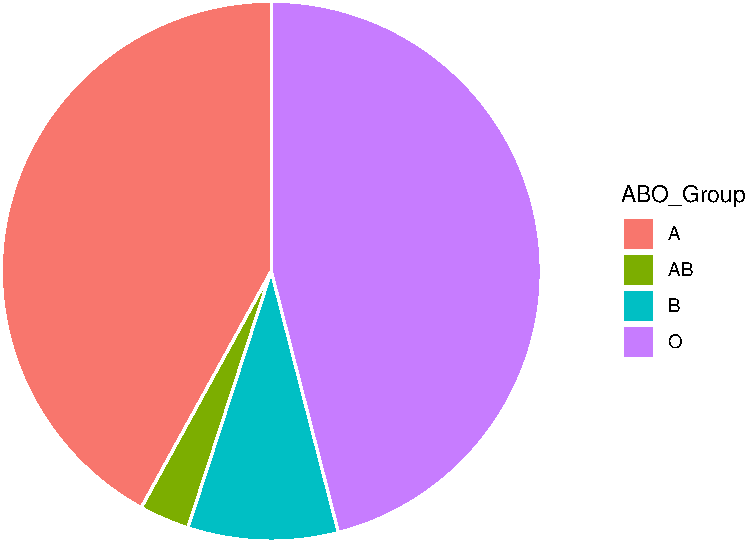
\includegraphics{forensic-statistics-book_files/figure-latex/pie-chart-1.pdf}
\caption{\label{fig:pie-chart}Relative Frequencies for ABO Blood Groups}
\end{figure}

Pie charts are effective for displaying the relative frequencies of a small
number of categories. They are not recommended, however, when you have a large
number of categories. Pie charts can also be confusing when they are used to
compare the outcomes of two different surveys or experiments. In an influential
book on the use of graphs, Edward Tufte asserted, ``The only worse design than
a pie chart is several of them.''

\hypertarget{bar-charts}{%
\section{Bar Charts}\label{bar-charts}}

Bar charts can also be used to represent frequencies of different categories.
A bar chart of the ABO frequencies is shown in Figure \ref{fig:bar-chart}.
Frequencies are shown
on the Y-axis and the blood group is shown on the X-axis.

\begin{figure}
\centering
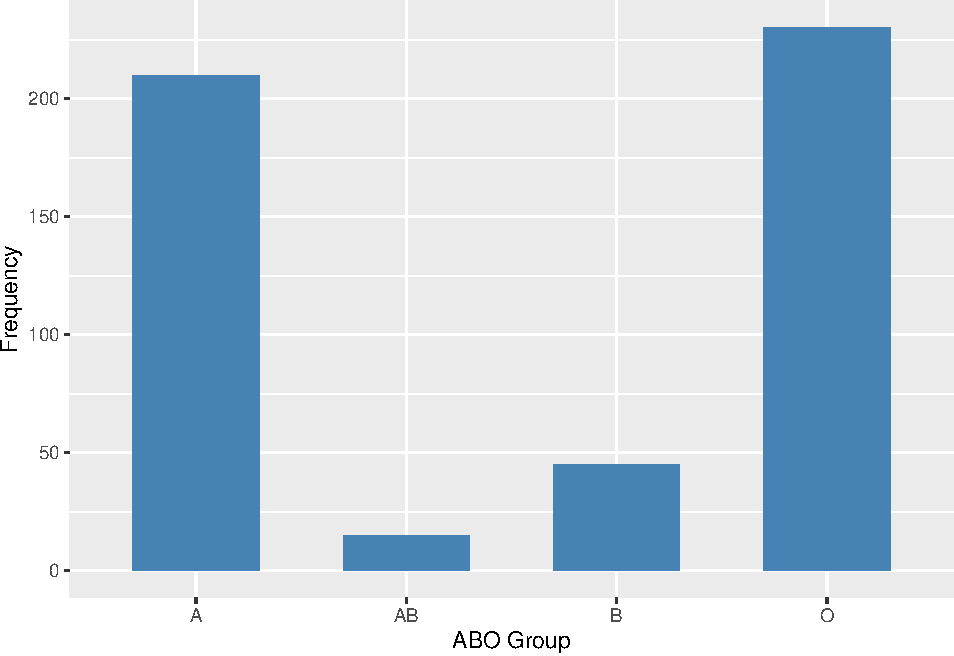
\includegraphics{forensic-statistics-book_files/figure-latex/bar-chart-1.pdf}
\caption{\label{fig:bar-chart}Frequencies for ABO Blood Groups}
\end{figure}

The Y-axis also can show the percentage of observations
instead of the number of observations, as in Figure \ref{fig:bar-chart-percent}.

\begin{figure}
\centering
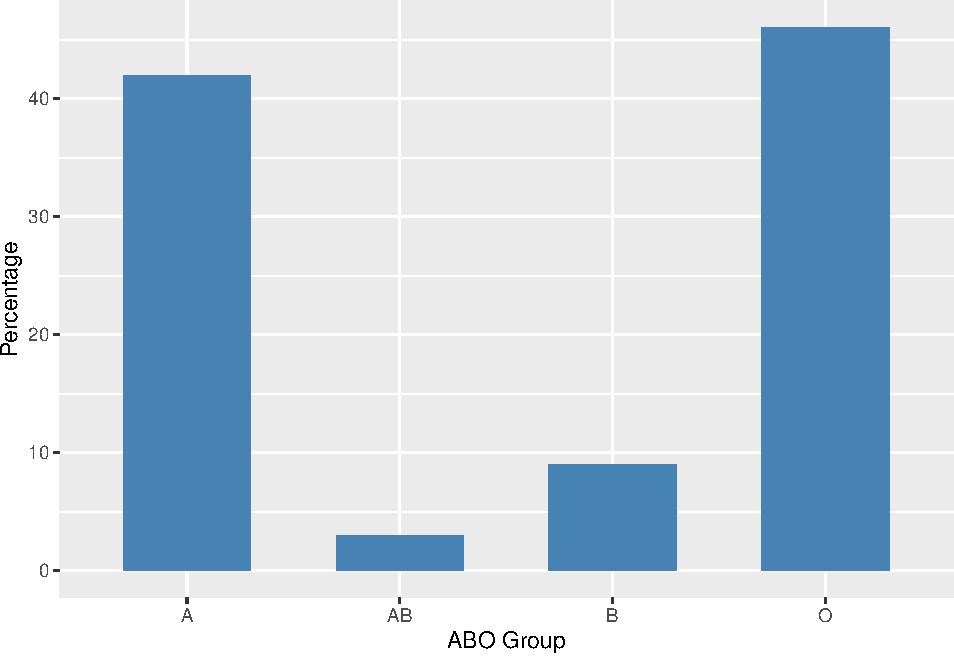
\includegraphics{forensic-statistics-book_files/figure-latex/bar-chart-percent-1.pdf}
\caption{\label{fig:bar-chart-percent}Percentages for ABO Blood Groups}
\end{figure}

\hypertarget{comparing-distributions}{%
\section{Comparing Distributions}\label{comparing-distributions}}

Often we need to compare different sets of data, or different subsets
within the same overall data set In this case, we are comparing the
``distributions'' of outcomes or responses. Bar charts are
often excellent for illustrating differences between two distributions. Table
2 shows the distribution (in percentages) of ABO blood groups for those in
Albania and Australia.

\[
\begin{array}{|c|c|c|} \hline
\text{ABO} && \\
\text{Group} & \text{Albania} & \text{Australia} \\ \hline
\mathrm{A} & 36.7 & 38.0 \\  \hline
\mathrm{B} & 17.1 & 10.0 \\  \hline
\mathrm{AB} & 6.1 & 3.0 \\  \hline
\mathrm{O} & 40.1 & 49.0 \\  \hline
\end{array}\\
\mbox{Table 2: ABO Blood Group Percentages}
\]
From Table 2 we see that ABO groups B and AB are more common in Albania,
group O is more common in Australia, and group A is similar for both.
This can be seen in the bar chart in Figure \ref{fig:horiz-bar}.

\begin{figure}
\centering
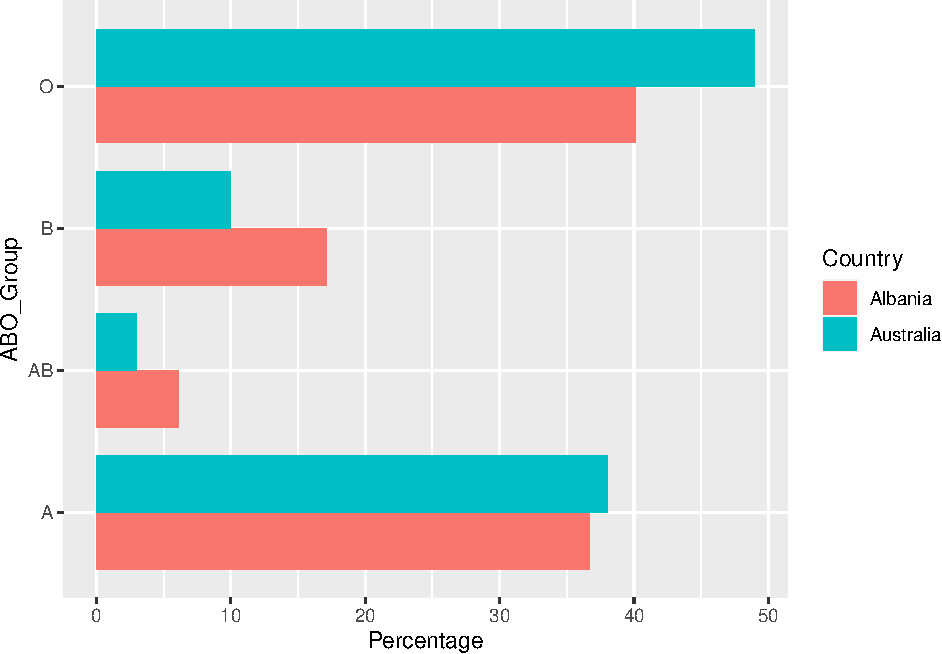
\includegraphics{forensic-statistics-book_files/figure-latex/horiz-bar-1.pdf}
\caption{\label{fig:horiz-bar}Percentages for ABO Blood Groups by Country}
\end{figure}

The bars in Figure \ref{fig:horiz-bar} are oriented horizontally rather than vertically. The
horizontal format is useful when you have many categories because there is more
room for the category labels.

\begin{center}\rule{0.5\linewidth}{0.5pt}\end{center}

\hypertarget{exercises-2}{%
\section{Exercises}\label{exercises-2}}

\begin{enumerate}
\def\labelenumi{\arabic{enumi}.}
\tightlist
\item
  \(\text{Put exercises here}\)
\end{enumerate}

\hypertarget{code-appendix}{%
\section{Code Appendix}\label{code-appendix}}

\begin{Shaded}
\begin{Highlighting}[]
\KeywordTok{library}\NormalTok{(dplyr)}
\KeywordTok{library}\NormalTok{(ggplot2)}
\KeywordTok{library}\NormalTok{(tidyr)}

\NormalTok{data <-}\StringTok{ }\KeywordTok{data.frame}\NormalTok{(}\DataTypeTok{ABO_Group =} \KeywordTok{c}\NormalTok{(}\StringTok{"A"}\NormalTok{, }\StringTok{"B"}\NormalTok{, }\StringTok{"AB"}\NormalTok{, }\StringTok{"O"}\NormalTok{), }\DataTypeTok{value =} \KeywordTok{c}\NormalTok{(}\DecValTok{210}\NormalTok{, }\DecValTok{45}\NormalTok{, }\DecValTok{15}\NormalTok{, }\DecValTok{230}\NormalTok{)) }\OperatorTok
\StringTok{  }\KeywordTok{mutate}\NormalTok{(}\DataTypeTok{prop =}\NormalTok{ value }\OperatorTok{/}\StringTok{ }\KeywordTok{sum}\NormalTok{(value) }\OperatorTok{*}\StringTok{ }\DecValTok{100}\NormalTok{)}

\CommentTok{# Figure 7.1 -----}
\KeywordTok{ggplot}\NormalTok{(}\DataTypeTok{data =}\NormalTok{ data, }\KeywordTok{aes}\NormalTok{(}\DataTypeTok{x =} \StringTok{""}\NormalTok{, }\DataTypeTok{y =}\NormalTok{ prop, }\DataTypeTok{fill =}\NormalTok{ ABO_Group)) }\OperatorTok{+}\StringTok{ }
\StringTok{  }\KeywordTok{geom_bar}\NormalTok{(}\DataTypeTok{stat =} \StringTok{"identity"}\NormalTok{, }\DataTypeTok{width =} \DecValTok{1}\NormalTok{, }\DataTypeTok{color =} \StringTok{"white"}\NormalTok{) }\OperatorTok{+}\StringTok{ }
\StringTok{  }\KeywordTok{coord_polar}\NormalTok{(}\StringTok{"y"}\NormalTok{, }\DataTypeTok{start =} \DecValTok{0}\NormalTok{) }\OperatorTok{+}\StringTok{ }
\StringTok{  }\KeywordTok{theme_void}\NormalTok{()}

\CommentTok{# Figure 7.2 -----}
\KeywordTok{ggplot}\NormalTok{(data, }\KeywordTok{aes}\NormalTok{(ABO_Group, value)) }\OperatorTok{+}\StringTok{ }
\StringTok{  }\KeywordTok{geom_bar}\NormalTok{(}\DataTypeTok{stat =} \StringTok{"identity"}\NormalTok{, }\DataTypeTok{fill =} \StringTok{"steelblue"}\NormalTok{) }\OperatorTok{+}\StringTok{ }
\StringTok{  }\KeywordTok{labs}\NormalTok{(}\DataTypeTok{x =} \StringTok{"ABO Group"}\NormalTok{, }\DataTypeTok{y =} \StringTok{"Frequency"}\NormalTok{)}

\CommentTok{# Figure 7.3 -----}
\KeywordTok{ggplot}\NormalTok{(data, }\KeywordTok{aes}\NormalTok{(ABO_Group, prop)) }\OperatorTok{+}\StringTok{ }
\StringTok{  }\KeywordTok{geom_bar}\NormalTok{(}\DataTypeTok{stat =} \StringTok{"identity"}\NormalTok{, }\DataTypeTok{fill =} \StringTok{"#B4464B"}\NormalTok{) }\OperatorTok{+}\StringTok{ }
\StringTok{  }\KeywordTok{labs}\NormalTok{(}\DataTypeTok{x =} \StringTok{"ABO Group"}\NormalTok{, }\DataTypeTok{y =} \StringTok{"Percentage"}\NormalTok{)}

\CommentTok{# Figure 7.4 -----}
\NormalTok{data <-}\StringTok{ }\KeywordTok{data.frame}\NormalTok{(}\DataTypeTok{ABO_Group =} \KeywordTok{c}\NormalTok{(}\StringTok{"A"}\NormalTok{, }\StringTok{"B"}\NormalTok{, }\StringTok{"AB"}\NormalTok{, }\StringTok{"O"}\NormalTok{), }
                   \DataTypeTok{Albania =} \KeywordTok{c}\NormalTok{(}\FloatTok{36.7}\NormalTok{, }\FloatTok{17.1}\NormalTok{, }\FloatTok{6.1}\NormalTok{, }\FloatTok{40.1}\NormalTok{), }
                   \DataTypeTok{Australia =} \KeywordTok{c}\NormalTok{(}\DecValTok{38}\NormalTok{, }\DecValTok{10}\NormalTok{, }\DecValTok{3}\NormalTok{, }\DecValTok{49}\NormalTok{)) }\OperatorTok
\StringTok{  }\KeywordTok{pivot_longer}\NormalTok{(}\OperatorTok{!}\NormalTok{ABO_Group, }\DataTypeTok{names_to =} \StringTok{"Country"}\NormalTok{, }\DataTypeTok{values_to =} \StringTok{"Percentage"}\NormalTok{)}

\KeywordTok{ggplot}\NormalTok{(data, }\KeywordTok{aes}\NormalTok{(ABO_Group, Percentage, }\DataTypeTok{fill =}\NormalTok{ Country)) }\OperatorTok{+}\StringTok{ }
\StringTok{  }\KeywordTok{geom_bar}\NormalTok{(}\DataTypeTok{stat =} \StringTok{"identity"}\NormalTok{, }\DataTypeTok{position =} \StringTok{"dodge"}\NormalTok{, }\DataTypeTok{width =} \FloatTok{0.8}\NormalTok{) }\OperatorTok{+}\StringTok{ }
\StringTok{  }\KeywordTok{labs}\NormalTok{(}\DataTypeTok{x =} \StringTok{"ABO Group"}\NormalTok{)}
  \KeywordTok{coord_flip}\NormalTok{()}
\end{Highlighting}
\end{Shaded}

\hypertarget{graphing-distributions-histograms}{%
\chapter{Graphing Distributions: Histograms}\label{graphing-distributions-histograms}}

Note: Portions below modeled after content from
\emph{Online Statistics Education: A Multimedia Course of Study}
(\url{http://onlinestatbook.com/}) Project Leader: David M. Lane, Rice University

\hypertarget{introduction-1}{%
\section{Introduction}\label{introduction-1}}

The ``distribution'' of a set of data consists of the set of possible data values and the
frequency that the values occur.
A \textbf{histogram} is a graphical method for displaying the shape of a distribution.
It is particularly useful when there are a large number of data values, when
it is not practical to list all values.

We begin with an example consisting of the weights of 371 bags containing a
substance suspected of being narcotics. The weights of the bags range from
215 to 270 grams. Below are the weights for 10 bags. (It is not
practical to show them all.)

\[
240.91, 234.66, 246.84, 244.24, 253.39, 245.07, 228.75, 237.29, 255.69, 254.64
\]

One way to get a sense of the distribution of the weights is through the
use of a frequency table, where we organize the data into groups of similar
weights and the count the number in each group. The results for this
data set are shown in Table 1.

\[
\begin{array}{|c|c|r|} \hline
\mathrm{Interval} & \mathrm{Interval} & \mathrm{Class}\hspace{.175in}\\
\text{Lower Limit} & \text{Upper Limit} & \mathrm{Frequency} \\ \hline
215 & 220 & 4\hspace{.3in} \\  \hline
220 & 225  & 8\hspace{.3in} \\  \hline
225 & 230 & 31\hspace{.3in} \\  \hline
230 & 235 & 74\hspace{.3in} \\  \hline
235 & 240 & 88\hspace{.3in} \\  \hline
240 & 245 & 75\hspace{.3in} \\  \hline
245 & 250 & 57\hspace{.3in} \\  \hline
250 & 255 & 25\hspace{.3in} \\  \hline
255 & 260 & 8\hspace{.3in} \\  \hline
260 & 265 & 1\hspace{.3in} \\  \hline
\end{array}\\
\mbox{Table 1: Grouped Frequency Distribution of Weights}
\]

To create this table, the range of weights was broken into \emph{class intervals}.
The first interval is from 215 to 220, the second from 220 to 225, and so on. Next, the number of weights
falling into each interval was counted to obtain the class frequencies. There are four weights\\
in the first interval, eight in the second, etc.

Class intervals of width 5 provide enough detail about the distribution to be revealing without
making the graph too ``choppy.'' How one goes about choosing the widths (called ``bin widths'') of
class intervals is discussed later in this section.

In a histogram the class frequencies are represented by bars, which provides a graphical
depiction of the data. The height of each bar corresponds
to its class frequency. A histogram of the weight data is shown in Figure \ref{fig:histogram}.

\begin{figure}
\centering
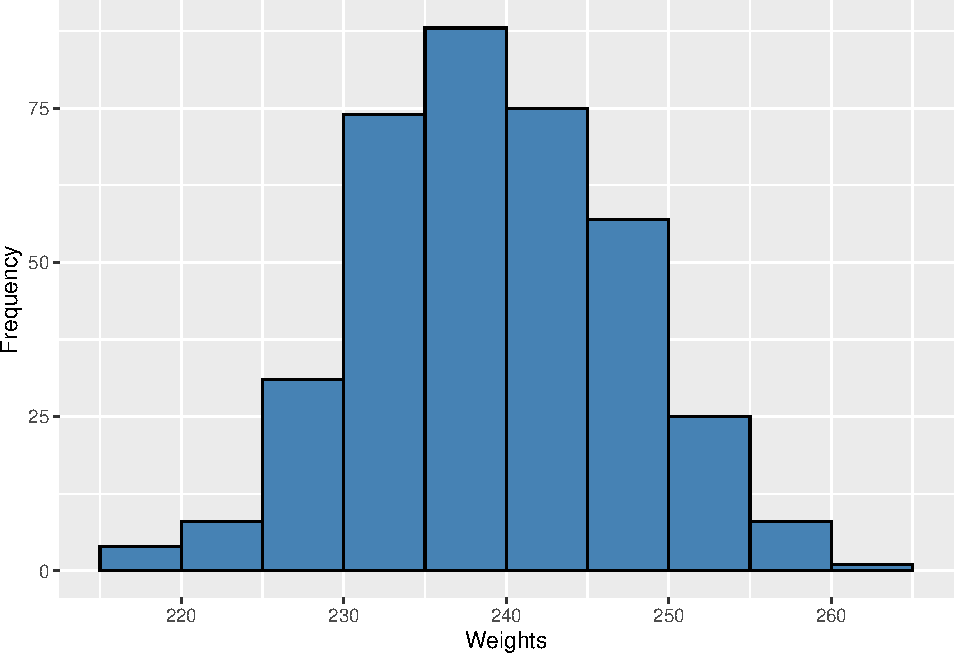
\includegraphics{forensic-statistics-book_files/figure-latex/histogram-1.pdf}
\caption{\label{fig:histogram}Histogram of Weights}
\end{figure}

We can see from the histogram that most of the weights are between 230 and 250 grams,
with fewer weights in the extremes. We can also see that the distribution is not
quite symmetric, the weights extend to the right farther than to the left. This
distribution is therefore said to be \emph{skewed}.

Because the weights are measured to two decimal
places, it is not likely that we get many ``fence-sitters'' -- that is, values
that land right on the border between two bins. This allows use to choose
whole numbers as boundaries, which avoids a cluttered appearance. Computer
software generally will use this option when feasible, and sometimes automatically
labels the middle of each interval instead of the endpoints.

Histograms can be based on relative frequencies instead of actual frequencies,
showing the proportion (or percentage) of values in each interval instead of
the exact frequence. Our weight data is displayed as percentages in
Figure \ref{fig:histogram-perc}. To get the percentages, we divide
each frequency by the number of data values (that gives the proportion), and
then multiply by 100 to convert to percentages.

\begin{figure}
\centering
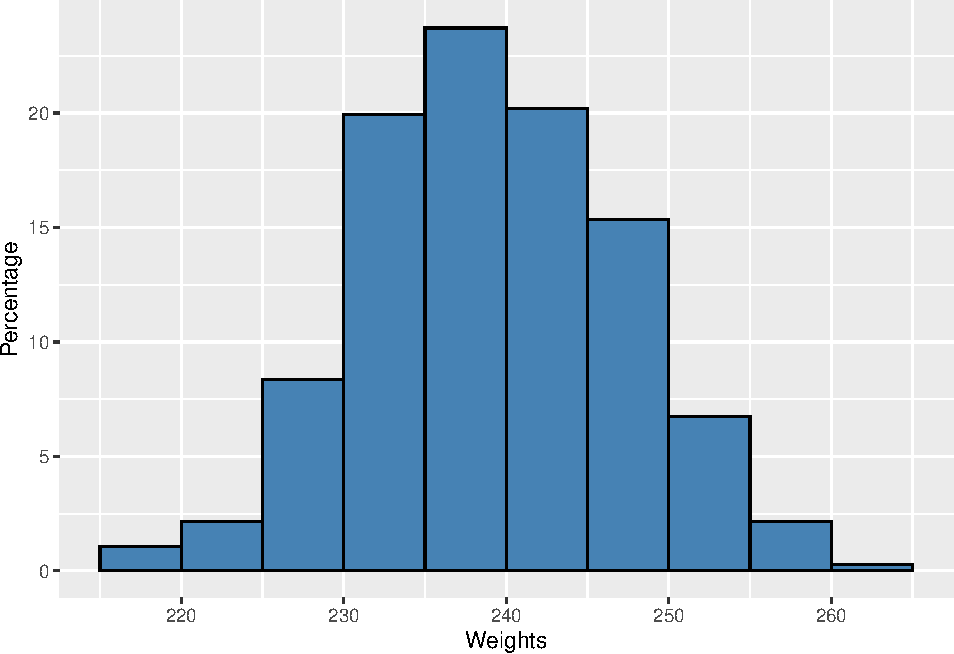
\includegraphics{forensic-statistics-book_files/figure-latex/histogram-perc-1.pdf}
\caption{\label{fig:histogram-perc}Histogram of Weights}
\end{figure}

We see that the shape of the histogram is unchanged, only the Y-axis is
different.

The choice of bin width determines the number of class intervals.
This decision, along with the choice of starting point for the first interval,
affects the shape of the histogram. In Figure \ref{fig:histogram-two} we see
histograms for our data using bins of width 1 (left) and width 10 (right).
These both give a general sense of the distribution, but here bins of width 1
produce a graph that is too busy while bins of width 10 produce a graph that
lacks detail.

\begin{figure}
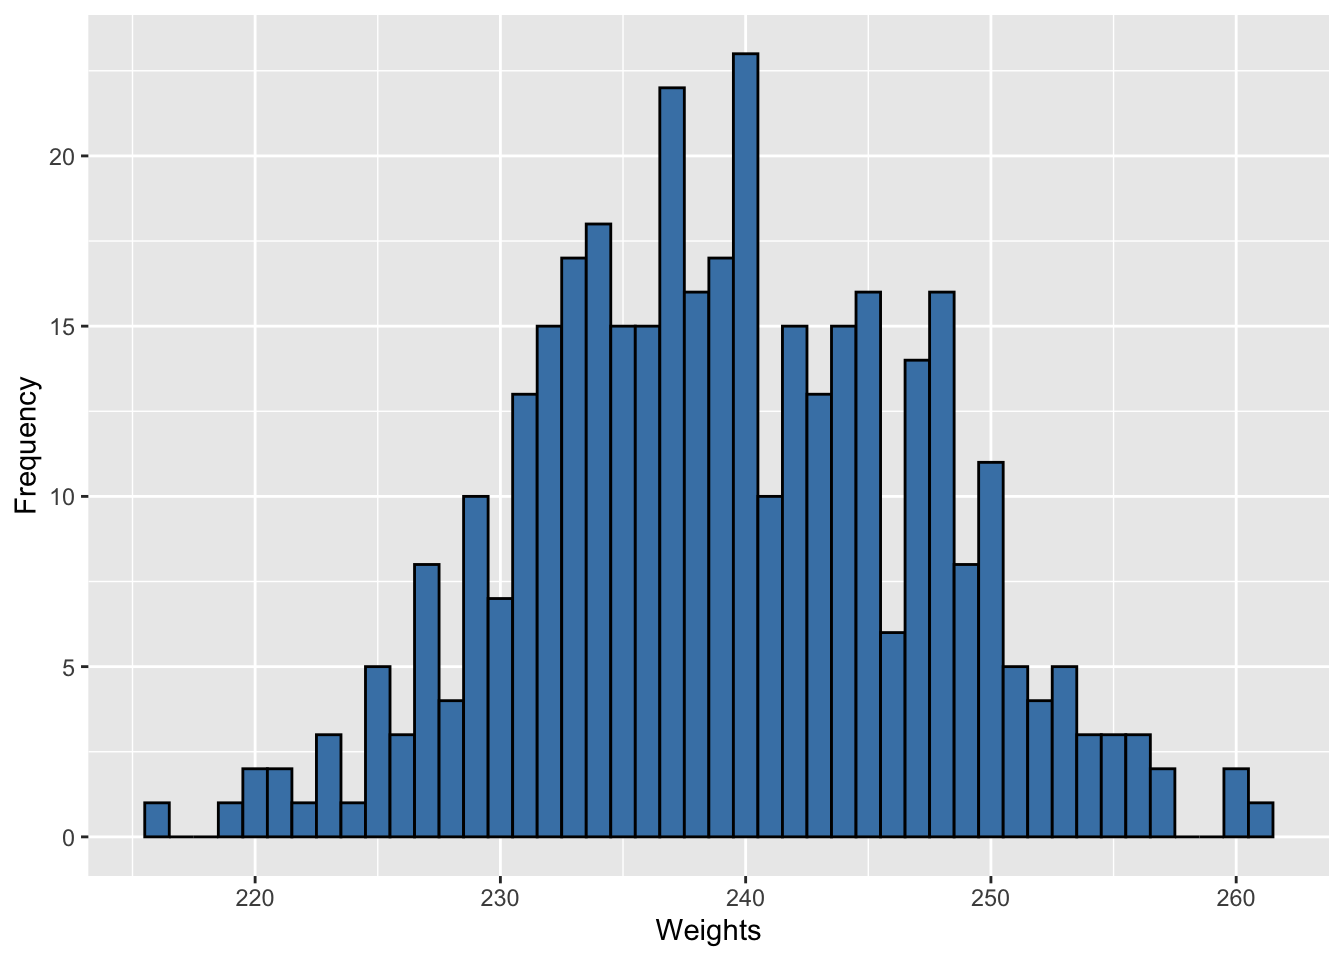
\includegraphics[width=0.5\linewidth]{forensic-statistics-book_files/figure-latex/histogram-two-1} 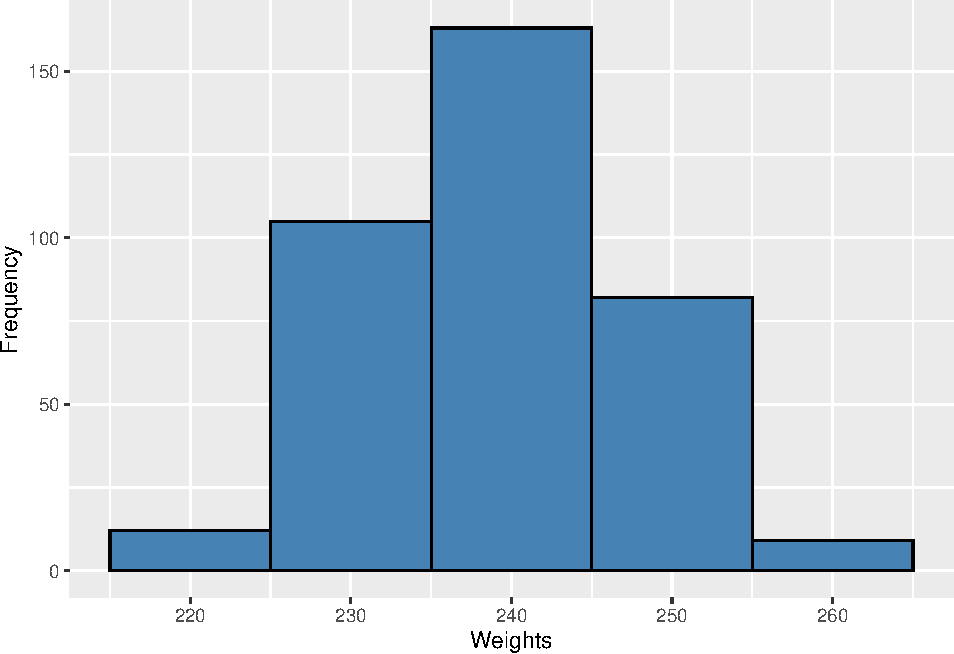
\includegraphics[width=0.5\linewidth]{forensic-statistics-book_files/figure-latex/histogram-two-2} \caption{Histograms with Different Bin Widths}\label{fig:histogram-two}
\end{figure}

Most software have defaults for bin widths that might work well for a given set
of data, or might not. There are some ``rules of thumb'' that can help guide
the choice of bin width but these are just guidelines that should not be
regarded as definitive, so do not feel bound to them. That said, here are
a couple of general guidelines you can consider:

\(\bullet\) Sturges' rule is to set the number of intervals as close as possible to
\(1 + \log_2(N)\), where \(\log_2(N)\) is the base 2 log of the number of
observations \(N\). For our data set of \(N = 371\), we have \(1 + \log_2(N) = 9.535\)
which suggests 10 intervals, which happens to match our choice.

\(\bullet\) The Rice rule suggests that the number of intervals should be the integer
nearest to \(2\sqrt[3]{N}\), twice the cube root of the number of data values.
For \(N = 371\) this formula gives \(2\sqrt[3]{371} = 14.371\), which is somewhat more
that we chose.

The above rules are just a guide, you are advised to experiment with different
numbers of intervals and choose the histogram that you feel best conveys the
shape of the distribution.

\begin{center}\rule{0.5\linewidth}{0.5pt}\end{center}

\hypertarget{exercises-3}{%
\section{Exercises}\label{exercises-3}}

\begin{enumerate}
\def\labelenumi{\arabic{enumi}.}
\tightlist
\item
  \(\text{Put exercises here}\)
\end{enumerate}

\hypertarget{code-appendix-1}{%
\section{Code Appendix}\label{code-appendix-1}}

\begin{Shaded}
\begin{Highlighting}[]
\KeywordTok{set.seed}\NormalTok{(}\DecValTok{4}\NormalTok{)}
\NormalTok{data01 <-}\StringTok{ }\KeywordTok{rnorm}\NormalTok{(}\DecValTok{371}\NormalTok{, }\DataTypeTok{mean =} \DecValTok{239}\NormalTok{, }\DataTypeTok{sd =} \DecValTok{8}\NormalTok{)}
\NormalTok{data01 <-}\StringTok{ }\KeywordTok{data.frame}\NormalTok{(}\DataTypeTok{Weights =} \KeywordTok{ifelse}\NormalTok{(data01 }\OperatorTok{>}\StringTok{ }\DecValTok{239}\NormalTok{, }\DecValTok{239} \OperatorTok{+}\StringTok{ }\FloatTok{1.1} \OperatorTok{*}\StringTok{ }\NormalTok{(data01 }\OperatorTok{-}\StringTok{ }\DecValTok{239}\NormalTok{), data01))}

\CommentTok{# Figure 8.1 -----}
\NormalTok{data01 }\OperatorTok\StringTok{ }\KeywordTok{ggplot}\NormalTok{() }\OperatorTok{+}\StringTok{ }
\StringTok{  }\KeywordTok{geom_histogram}\NormalTok{(}\KeywordTok{aes}\NormalTok{(}\DataTypeTok{x =}\NormalTok{ Weights), }\DataTypeTok{breaks =} \KeywordTok{seq}\NormalTok{(}\DecValTok{215}\NormalTok{, }\DecValTok{265}\NormalTok{, }\DataTypeTok{by =} \DecValTok{5}\NormalTok{), }
                 \DataTypeTok{fill =} \StringTok{"steelblue"}\NormalTok{, }\DataTypeTok{color =} \StringTok{"black"}\NormalTok{) }\OperatorTok{+}\StringTok{ }
\StringTok{  }\KeywordTok{labs}\NormalTok{(}\DataTypeTok{y =} \StringTok{"Frequency"}\NormalTok{)}

\CommentTok{# Figure 8.2 -----}
\NormalTok{data01 }\OperatorTok\StringTok{ }\KeywordTok{ggplot}\NormalTok{() }\OperatorTok{+}\StringTok{ }
\StringTok{  }\KeywordTok{geom_histogram}\NormalTok{(}\KeywordTok{aes}\NormalTok{(}\DataTypeTok{x =}\NormalTok{ Weights, }\DataTypeTok{y =} \DecValTok{100} \OperatorTok{*}\StringTok{ }\NormalTok{..count.. }\OperatorTok{/}\StringTok{ }\KeywordTok{sum}\NormalTok{(count)), }
                 \DataTypeTok{breaks =} \KeywordTok{seq}\NormalTok{(}\DecValTok{215}\NormalTok{, }\DecValTok{265}\NormalTok{, }\DataTypeTok{by =} \DecValTok{5}\NormalTok{), }
                 \DataTypeTok{fill =} \StringTok{"steelblue"}\NormalTok{, }\DataTypeTok{color =} \StringTok{"black"}\NormalTok{) }\OperatorTok{+}\StringTok{ }
\StringTok{  }\KeywordTok{labs}\NormalTok{(}\DataTypeTok{y =} \StringTok{"Percentage"}\NormalTok{)}

\CommentTok{# Figure 8.3 -----}
\NormalTok{data01 }\OperatorTok\StringTok{ }\KeywordTok{ggplot}\NormalTok{() }\OperatorTok{+}\StringTok{ }
\StringTok{  }\KeywordTok{geom_histogram}\NormalTok{(}\KeywordTok{aes}\NormalTok{(}\DataTypeTok{x =}\NormalTok{ Weights), }\DataTypeTok{binwidth =} \DecValTok{1}\NormalTok{, }\DataTypeTok{fill =} \StringTok{"steelblue"}\NormalTok{, }\DataTypeTok{color =} \StringTok{"black"}\NormalTok{) }\OperatorTok{+}\StringTok{ }
\StringTok{  }\KeywordTok{labs}\NormalTok{(}\DataTypeTok{y =} \StringTok{"Frequency"}\NormalTok{)}

\NormalTok{data01 }\OperatorTok\StringTok{ }\KeywordTok{ggplot}\NormalTok{() }\OperatorTok{+}\StringTok{ }
\StringTok{  }\KeywordTok{geom_histogram}\NormalTok{(}\KeywordTok{aes}\NormalTok{(}\DataTypeTok{x =}\NormalTok{ Weights), }\DataTypeTok{binwidth =} \DecValTok{10}\NormalTok{, }\DataTypeTok{fill =} \StringTok{"steelblue"}\NormalTok{, }\DataTypeTok{color =} \StringTok{"black"}\NormalTok{) }\OperatorTok{+}\StringTok{ }
\StringTok{  }\KeywordTok{labs}\NormalTok{(}\DataTypeTok{y =} \StringTok{"Frequency"}\NormalTok{)}
\end{Highlighting}
\end{Shaded}

\hypertarget{graphing-distributions-box-plots}{%
\chapter{Graphing Distributions: Box Plots}\label{graphing-distributions-box-plots}}

Note: Portions below modeled after content from
\emph{Online Statistics Education: A Multimedia Course of Study}
(\url{http://onlinestatbook.com/}) Project Leader: David M. Lane, Rice University

\hypertarget{basic-box-plots}{%
\section{Basic box plots}\label{basic-box-plots}}

In this chapter we discuss the \emph{box plot} which provides a useful way to graphically
display information about the distribution of a set of data,
identify outliers, and compare distributions.

To get us started, suppose that we have small pieces of glass from two different
sources: a broken window at the scene of a burglary and the trunk of a car
belonging to a suspect. To compare the glass from the two sources, a trace
element present in glass can be measured. The amount present varies within
a sheet of glass so measurements are taken from numerous pieces found at the
crime scene and in the car trunk. (The specifics of the element and measurement
units are not important for this discussion.) The measurements are given below:

Car Trunk: 67.9, 68.9, 69.5, 67.6, 73.4, 64.5, 73.0, 59.7, 66.9, 68.2, 71.8, 64.8, 56.3

Crime Scene: 55.6, 65.6, 68.0, 68.9, 67.7, 66.5, 66.8, 60.3, 68.0, 71.6, 61.4, 63.2, 68.2, 64.1, 64.8

To construct the box plot, we start by finding the 25th, 50th, and 75th percentiles
for each of our data sets. Recall that the 25th percentile is the quantity such
that 25\% of the data values are less than this quantity, and similarly for the
other percentiles. The percentiles for each of our data sets are shown in
Table 1.

\[
\begin{array}{|c|c|c|} \hline
& \mathrm{Car} & \text{Crime}  \\
\text{Percentile} & \mathrm{Trunk} & \text{Scene}  \\ \hline
25^{\text{th}} & 64.80 & 63.65  \\  \hline
50^{\text{th}}  & 67.90 & 66.50  \\  \hline
75^{\text{th}} & 69.50 & 68.00  \\  \hline
\end{array}\\
\mbox{Table 1: Percentiles}
\]

Figure \ref{fig:boxplot1} shows how these percentiles
are incorporated into box plots. The lower and upper
limits of the box (called ``hinges'') extend from the
25th to 75th percentile and a line between those at the 50th percentile
(which is the median).

\begin{figure}
\centering
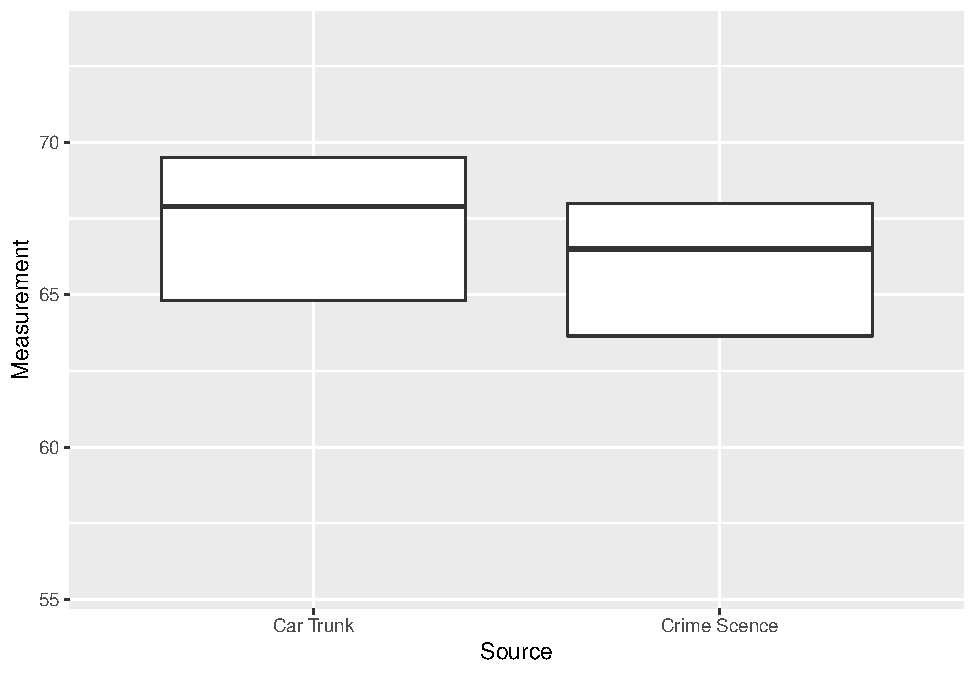
\includegraphics{forensic-statistics-book_files/figure-latex/boxplot1-1.pdf}
\caption{\label{fig:boxplot1}Box Plots of Glass Measurements}
\end{figure}

Comparing box plots, we see that the percentiles for the car trunk data
are somewhat greater than for the crime scene data but there is considerable
overlap between them. Based on this, it is difficult to say whether the
glass pieces from car trunk and crime scene are from the same
original source or different sources.

Most box plots have more information than that shown in Figure \ref{fig:boxplot1}
and there are a wide variety of options that can be included. We give a few
examples below to provide a sense of what is possible but these are by no means
comprehensive.

We next add ``whiskers'' above and below each box to give additional information
about the spread of the data. Whiskers are vertical lines that (optionally)
end in a horizontal stroke. Define the ``step'' to be 1.5 times the
IQR = 75th percentile - 25th percentile (IQR = ``Interquartile range'').
The upper whisker extends
from the upper hinge to the greatest data value that is less than one ``step''
above the upper hinge, with the lower whisker similarly defined. (Software
automates the process so one need not do this by hand.)

Figure \ref{fig:boxplot2} shows the box plots with whiskers.

\begin{figure}
\centering
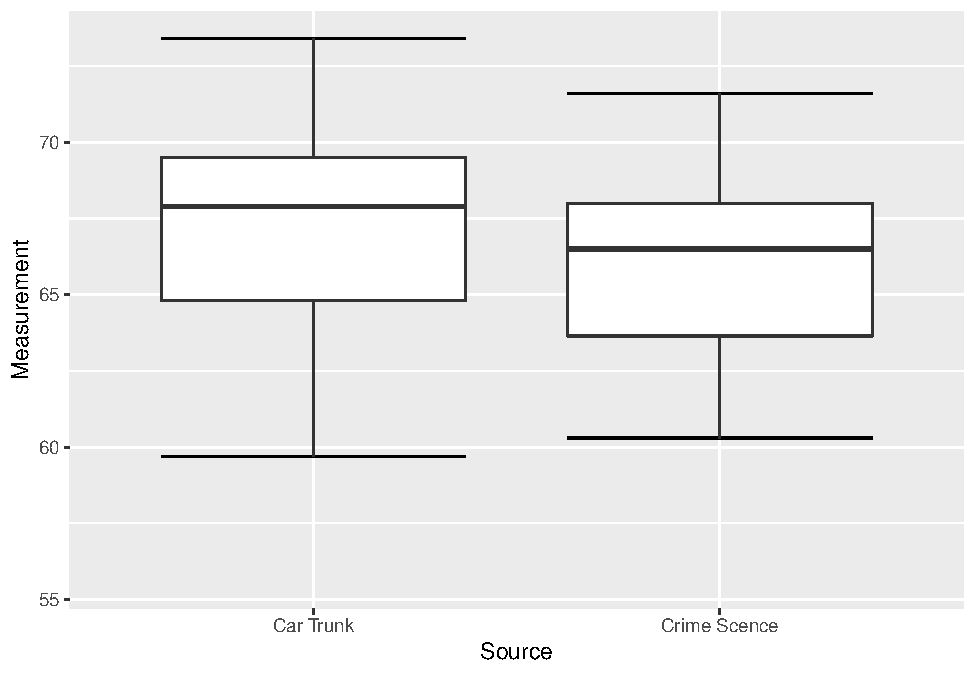
\includegraphics{forensic-statistics-book_files/figure-latex/boxplot2-1.pdf}
\caption{\label{fig:boxplot2}Box Plots of Glass Measurements}
\end{figure}

The whiskers add additional information about the spread of data, but do
not extend to all values. We indicate these with dots that are beyond
the whiskers in positions corresponding to data values. This is shown in
Figure \ref{fig:boxplot3}.

\begin{figure}
\centering
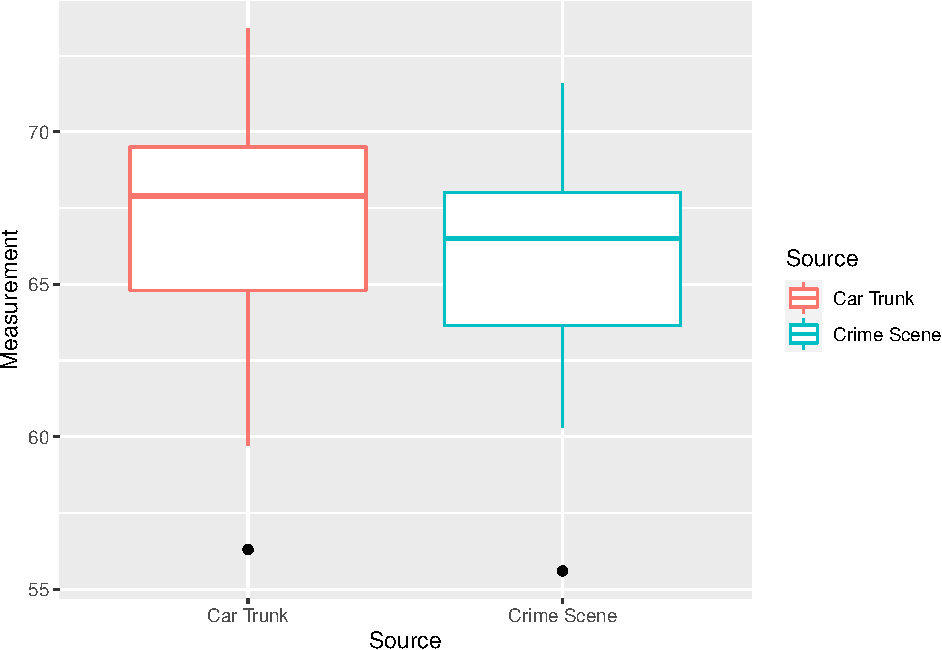
\includegraphics{forensic-statistics-book_files/figure-latex/boxplot3-1.pdf}
\caption{\label{fig:boxplot3}Box Plots of Glass Measurements}
\end{figure}

Some (but not all!) box plots also include a mark indicating the location of
the mean. This is added in Figure \ref{fig:boxplot4} as a red dot in each
box plot.

\begin{figure}
\centering
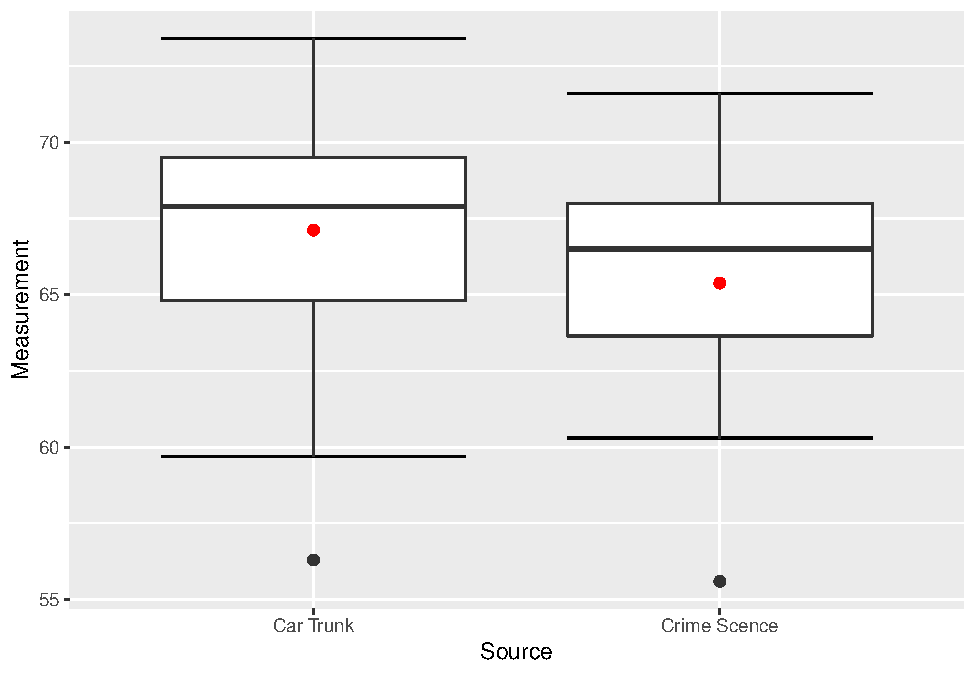
\includegraphics{forensic-statistics-book_files/figure-latex/boxplot4-1.pdf}
\caption{\label{fig:boxplot4}Box Plots of Glass Measurements}
\end{figure}

Figure \ref{fig:boxplot4} provides a good summary of the data. Half of
the scores in a distribution are between the hinges (recall that the hinges are
the 25th and 75th percentiles), we see that half the measurements for the glass
from the car trunk are between about 65 and 69, while the measurements from the
crime scene are between about 63.5 and 68. The IQR for each is about the same
but the overall range for the car trunk measurements is somewhat greater
then the crime scene measurements. For both data sets the mean is less than
the median, which is to be expected due to the extreme small values displayed
in Figure \ref{fig:boxplot4}.

\hypertarget{variations-on-box-plots}{%
\section{Variations on box plots}\label{variations-on-box-plots}}

Statistical analysis programs typically offer numerous options for creating
box plots. For instance, Figure \ref{fig:boxplot5} shows the box plots
as above but also includes the individual measurements along the vertical
axis. (The means are still red to distinguish it from the data values.)
This provides more detail on our data -- note the points that specify
the ends of the whiskers as well as the difference in how the points are
distributed within the boxes.

\begin{figure}
\centering
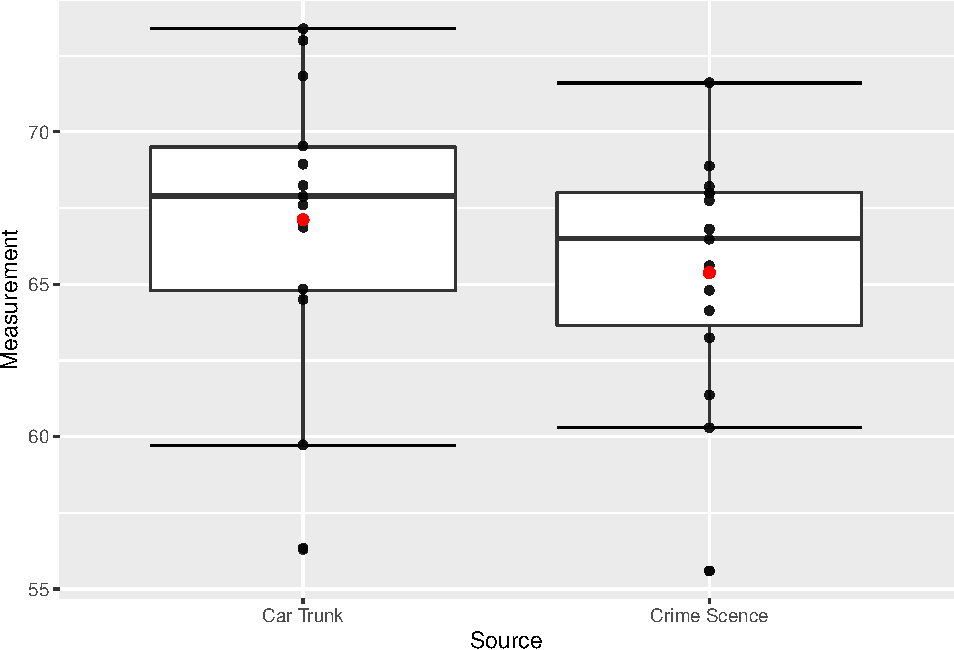
\includegraphics{forensic-statistics-book_files/figure-latex/boxplot5-1.pdf}
\caption{\label{fig:boxplot5}Box Plots of Glass Measurements}
\end{figure}

Showing the specific data values on the vertical axis works well as long as there
are not too many points and they do not tend to stack on top of each other.
In the case of more points and more repetition of values, an option that can
work is ``jittering'' which adds a horizontal offset so that points can be
distinguished. Figure \ref{fig:boxplot6} shows our data with a modest
amount of jitter added.

\begin{figure}
\centering
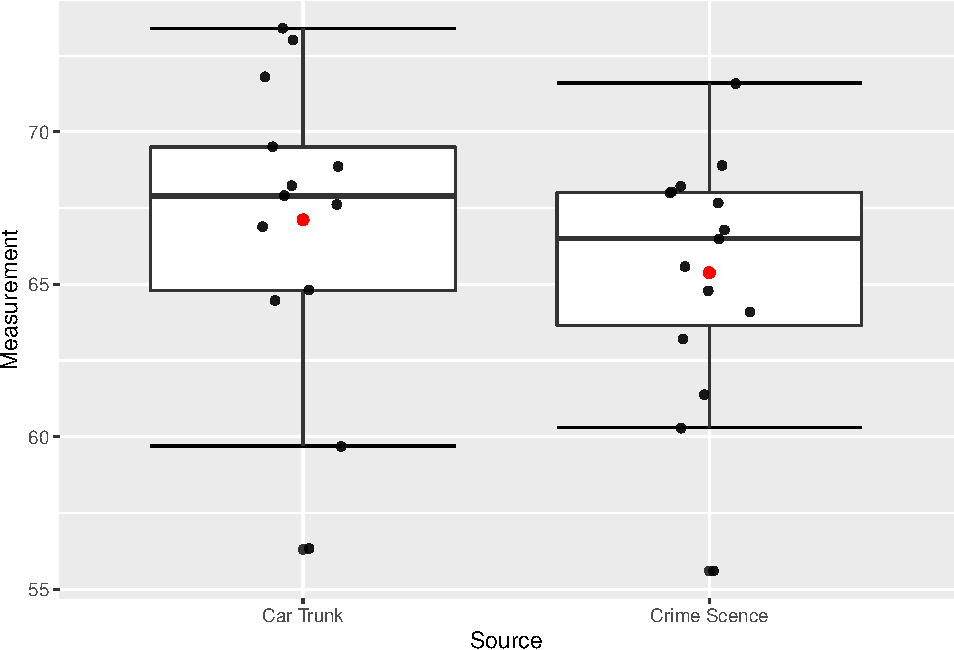
\includegraphics{forensic-statistics-book_files/figure-latex/boxplot6-1.pdf}
\caption{\label{fig:boxplot6}Box Plots of Glass Measurements}
\end{figure}

Different styles of box plots are best for different situations, and there are
no firm rules for which to use. When exploring your data, you should try several
ways of visualizing them. Which graphs you include in your report should depend
on how well different graphs reveal the aspects of the data you consider most
important.

\begin{center}\rule{0.5\linewidth}{0.5pt}\end{center}

\hypertarget{exercises-4}{%
\section{Exercises}\label{exercises-4}}

\begin{enumerate}
\def\labelenumi{\arabic{enumi}.}
\tightlist
\item
  \(\text{Put exercises here}\)
\end{enumerate}

\hypertarget{code-appendix-2}{%
\section{Code Appendix}\label{code-appendix-2}}

\begin{Shaded}
\begin{Highlighting}[]
\NormalTok{data01 <-}\StringTok{ }\KeywordTok{c}\NormalTok{(}\FloatTok{55.6}\NormalTok{, }\FloatTok{65.6}\NormalTok{, }\FloatTok{68.0}\NormalTok{, }\FloatTok{68.9}\NormalTok{, }\FloatTok{67.7}\NormalTok{, }\FloatTok{66.5}\NormalTok{, }\FloatTok{66.8}\NormalTok{, }\FloatTok{60.3}\NormalTok{, }\FloatTok{68.0}\NormalTok{, }\FloatTok{71.6}\NormalTok{, }\FloatTok{61.4}\NormalTok{, }\FloatTok{63.2}\NormalTok{, }\FloatTok{68.2}\NormalTok{, }\FloatTok{64.1}\NormalTok{, }\FloatTok{64.8}\NormalTok{)}
\NormalTok{data02 <-}\StringTok{ }\KeywordTok{c}\NormalTok{(}\FloatTok{67.9}\NormalTok{, }\FloatTok{68.9}\NormalTok{, }\FloatTok{69.5}\NormalTok{, }\FloatTok{67.6}\NormalTok{, }\FloatTok{73.4}\NormalTok{, }\FloatTok{64.5}\NormalTok{, }\FloatTok{73.0}\NormalTok{, }\FloatTok{59.7}\NormalTok{, }\FloatTok{66.9}\NormalTok{, }\FloatTok{68.2}\NormalTok{, }\FloatTok{71.8}\NormalTok{, }\FloatTok{64.8}\NormalTok{, }\FloatTok{56.3}\NormalTok{)}

\NormalTok{data01 <-}\StringTok{ }\KeywordTok{data.frame}\NormalTok{(}\DataTypeTok{Measurement =}\NormalTok{ data01, }\DataTypeTok{Source =} \StringTok{"Crime Scence"}\NormalTok{)}
\NormalTok{data02 <-}\StringTok{ }\KeywordTok{data.frame}\NormalTok{(}\DataTypeTok{Measurement =}\NormalTok{ data02, }\DataTypeTok{Source =} \StringTok{"Car Trunk"}\NormalTok{)}
\NormalTok{data03 <-}\StringTok{ }\KeywordTok{rbind}\NormalTok{(data01, data02)}

\CommentTok{# Figure 9.1 -----}
\NormalTok{data03 }\OperatorTok\StringTok{ }\KeywordTok{ggplot}\NormalTok{(}\KeywordTok{aes}\NormalTok{(}\DataTypeTok{x =}\NormalTok{ Source, }\DataTypeTok{y =}\NormalTok{ Measurement)) }\OperatorTok{+}
\StringTok{  }\KeywordTok{geom_boxplot}\NormalTok{(}\DataTypeTok{outlier.shape =} \OtherTok{NA}\NormalTok{, }\DataTypeTok{coef =} \DecValTok{0}\NormalTok{)}

\CommentTok{# Figure 9.2 -----}
\NormalTok{data03 }\OperatorTok\StringTok{ }\KeywordTok{ggplot}\NormalTok{(}\KeywordTok{aes}\NormalTok{(}\DataTypeTok{x =}\NormalTok{ Source, }\DataTypeTok{y =}\NormalTok{ Measurement)) }\OperatorTok{+}\StringTok{ }\KeywordTok{stat_boxplot}\NormalTok{(}\DataTypeTok{geom =} \StringTok{"errorbar"}\NormalTok{) }\OperatorTok{+}\StringTok{ }
\StringTok{  }\KeywordTok{geom_boxplot}\NormalTok{(}\DataTypeTok{outlier.shape =} \OtherTok{NA}\NormalTok{)}

\CommentTok{# Figure 9.3 -----}
\NormalTok{data03 }\OperatorTok\StringTok{ }\KeywordTok{ggplot}\NormalTok{(}\KeywordTok{aes}\NormalTok{(}\DataTypeTok{x =}\NormalTok{ Source, }\DataTypeTok{y =}\NormalTok{ Measurement)) }\OperatorTok{+}\StringTok{ }\KeywordTok{stat_boxplot}\NormalTok{(}\DataTypeTok{geom =} \StringTok{"errorbar"}\NormalTok{) }\OperatorTok{+}\StringTok{ }
\StringTok{  }\KeywordTok{geom_boxplot}\NormalTok{()}

\CommentTok{# Figure 9.4 -----}
\NormalTok{data03 }\OperatorTok\StringTok{ }\KeywordTok{ggplot}\NormalTok{(}\KeywordTok{aes}\NormalTok{(}\DataTypeTok{x =}\NormalTok{ Source, }\DataTypeTok{y =}\NormalTok{ Measurement)) }\OperatorTok{+}\StringTok{ }\KeywordTok{stat_boxplot}\NormalTok{(}\DataTypeTok{geom =} \StringTok{"errorbar"}\NormalTok{) }\OperatorTok{+}
\StringTok{  }\KeywordTok{geom_boxplot}\NormalTok{(}\DataTypeTok{outlier.size =} \DecValTok{2}\NormalTok{) }\OperatorTok{+}\StringTok{ }
\StringTok{  }\KeywordTok{stat_summary}\NormalTok{(}\DataTypeTok{fun =}\NormalTok{ mean, }\DataTypeTok{geom =} \StringTok{"point"}\NormalTok{, }\DataTypeTok{color =} \StringTok{"red"}\NormalTok{, }\DataTypeTok{size =} \DecValTok{2}\NormalTok{)}

\CommentTok{# Figure 9.5 -----}
\NormalTok{data03 }\OperatorTok\StringTok{ }\KeywordTok{ggplot}\NormalTok{(}\KeywordTok{aes}\NormalTok{(}\DataTypeTok{x =}\NormalTok{ Source, }\DataTypeTok{y =}\NormalTok{ Measurement)) }\OperatorTok{+}\StringTok{ }\KeywordTok{stat_boxplot}\NormalTok{(}\DataTypeTok{geom =} \StringTok{"errorbar"}\NormalTok{) }\OperatorTok{+}\StringTok{ }
\StringTok{  }\KeywordTok{geom_boxplot}\NormalTok{() }\OperatorTok{+}\StringTok{ }\KeywordTok{geom_jitter}\NormalTok{(}\DataTypeTok{width =} \DecValTok{0}\NormalTok{, }\DataTypeTok{alpha =} \FloatTok{0.9}\NormalTok{) }\OperatorTok{+}\StringTok{ }
\StringTok{  }\KeywordTok{stat_summary}\NormalTok{(}\DataTypeTok{fun =}\NormalTok{ mean, }\DataTypeTok{geom =} \StringTok{"point"}\NormalTok{, }\DataTypeTok{color =} \StringTok{"red"}\NormalTok{, }\DataTypeTok{size =} \DecValTok{2}\NormalTok{)}

\CommentTok{# Figure 9.6 -----}
\NormalTok{data03 }\OperatorTok\StringTok{ }\KeywordTok{ggplot}\NormalTok{(}\KeywordTok{aes}\NormalTok{(}\DataTypeTok{x =}\NormalTok{ Source, }\DataTypeTok{y =}\NormalTok{ Measurement)) }\OperatorTok{+}\StringTok{ }\KeywordTok{stat_boxplot}\NormalTok{(}\DataTypeTok{geom =} \StringTok{"errorbar"}\NormalTok{) }\OperatorTok{+}\StringTok{ }
\StringTok{  }\KeywordTok{geom_boxplot}\NormalTok{() }\OperatorTok{+}\StringTok{ }\KeywordTok{geom_jitter}\NormalTok{(}\DataTypeTok{width =} \FloatTok{0.1}\NormalTok{, }\DataTypeTok{alpha =} \FloatTok{0.9}\NormalTok{) }\OperatorTok{+}\StringTok{ }
\StringTok{  }\KeywordTok{stat_summary}\NormalTok{(}\DataTypeTok{fun =}\NormalTok{ mean, }\DataTypeTok{geom =} \StringTok{"point"}\NormalTok{, }\DataTypeTok{color =} \StringTok{"red"}\NormalTok{, }\DataTypeTok{size =} \DecValTok{2}\NormalTok{)}
\end{Highlighting}
\end{Shaded}

\hypertarget{graphing-distributions-bar-charts}{%
\chapter{Graphing Distributions: Bar Charts}\label{graphing-distributions-bar-charts}}

Note: Portions below modeled after content from
\emph{Online Statistics Education: A Multimedia Course of Study}
(\url{http://onlinestatbook.com/}) Project Leader: David M. Lane, Rice University

In the section on qualitative variables, we saw how bar charts can be used
to illustrate the frequencies (or relative frequencies) of different categories.
For example, the bar chart shown in Figure \ref{fig:bar-chart-percent2}
depicts the percentage of people in a population that have each of the four
possible ABO blood groups.

\begin{figure}
\centering
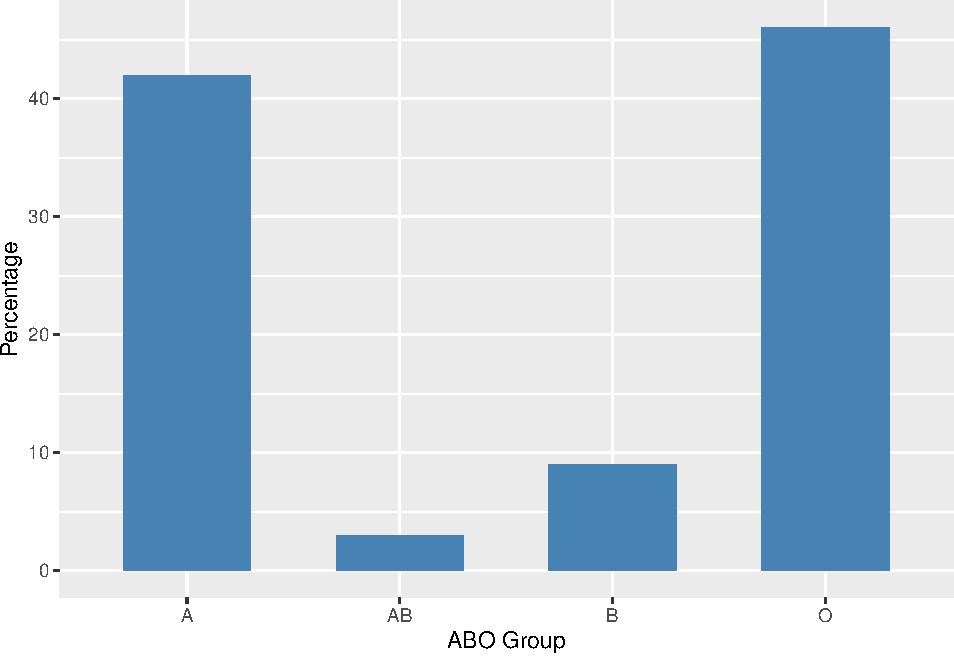
\includegraphics{forensic-statistics-book_files/figure-latex/bar-chart-percent2-1.pdf}
\caption{\label{fig:bar-chart-percent2}Percentages for ABO Blood Groups}
\end{figure}

In this chapter we consider how bar charts can be used to present other
types of quantitative information. The bar chart in Figure \ref{fig:bar-chart2}
presents the number of murders in four large U.S. cities.

\begin{figure}
\centering
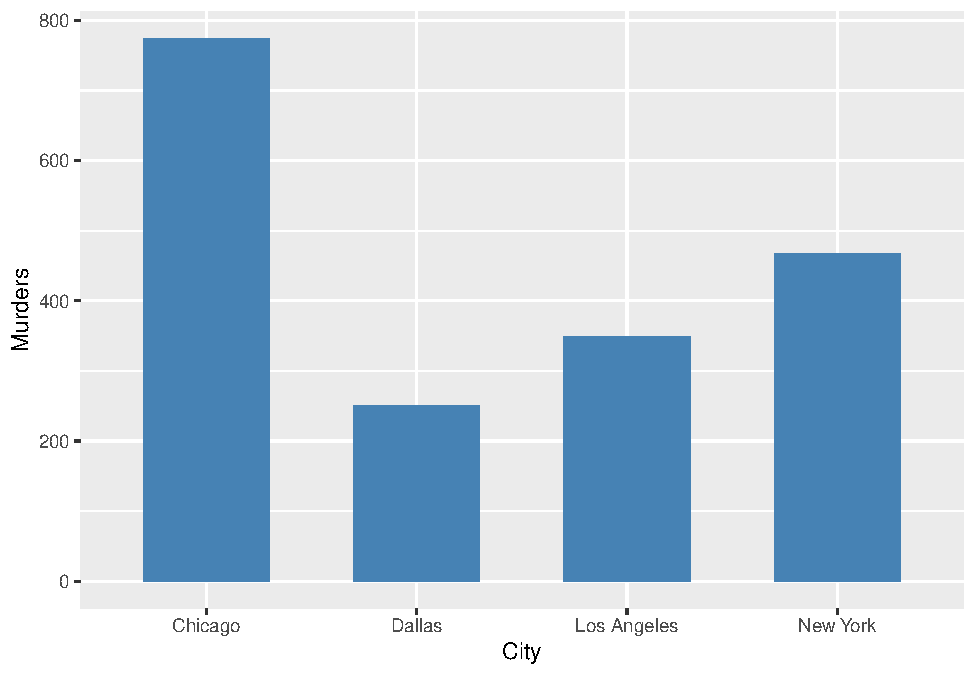
\includegraphics{forensic-statistics-book_files/figure-latex/bar-chart2-1.pdf}
\caption{\label{fig:bar-chart2}Number of murders, selected U.S. cities, year 2000}
\end{figure}

A case can be made that more relevant than the total number of murders is
the per capita number of murders. Figure \ref{fig:bar-chart3} gives the
number of murders per 1,000,000 population for the same cities.

\begin{figure}
\centering
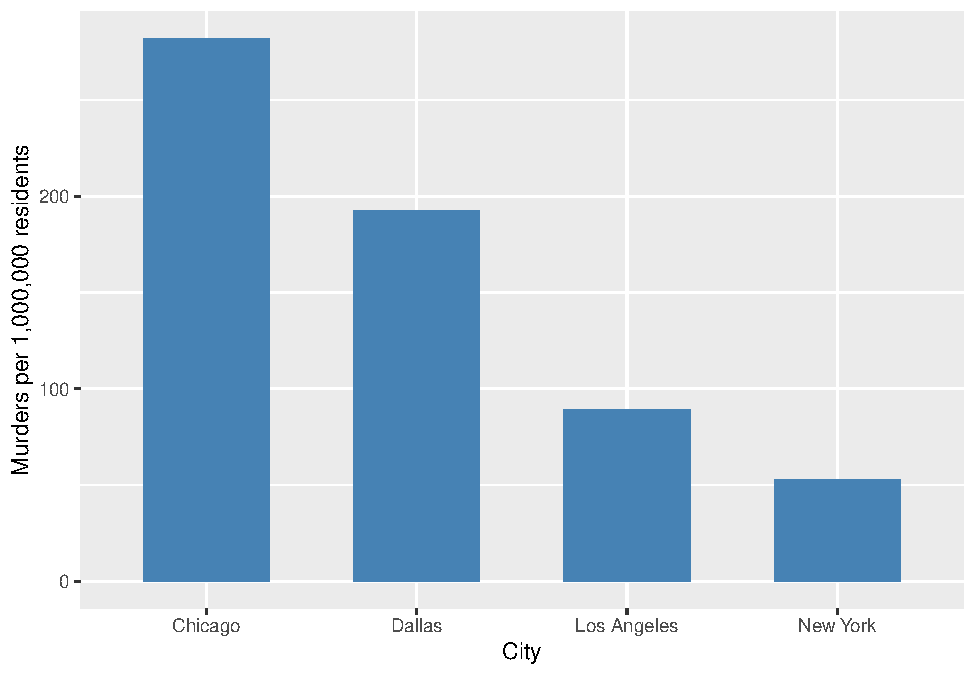
\includegraphics{forensic-statistics-book_files/figure-latex/bar-chart3-1.pdf}
\caption{\label{fig:bar-chart3}Murders per 1,000,000 residents, selected U.S. cities, year 2000}
\end{figure}

Bar charts can be useful for showing change over time. Figure \ref{fig:bar-chart4},
shows the year-to-year percent change in the number of shootings in the city of
Toronto. The considerable variation from one year to the next is clear. Note also
that negative percentages are possible, the result of the number of shootings
decreasing from one year to the next.

\begin{figure}
\centering
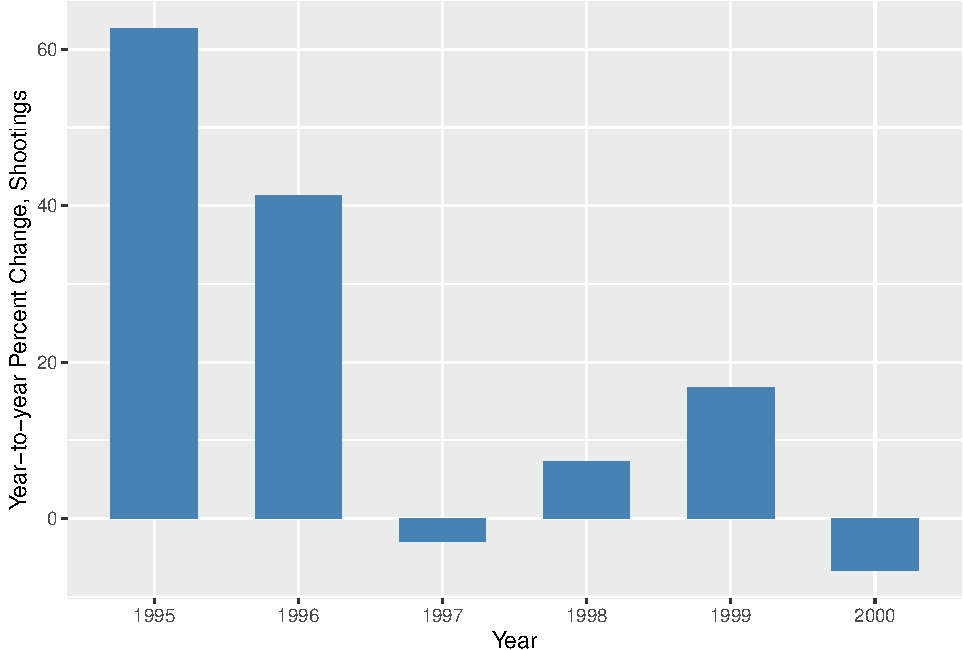
\includegraphics{forensic-statistics-book_files/figure-latex/bar-chart4-1.pdf}
\caption{\label{fig:bar-chart4}Year-to-year Percent Change, Shootings in Toronto}
\end{figure}

Bar charts are often used to compare the means of different experimental
conditions. Figure \ref{fig:bar-chart5} shows the mean trace element
measurement for collections of glass pieces found at a crime scene and
in the car trunk of a suspect. (This data is treated more thoroughly
in the chapter on box plots.)

\begin{figure}
\centering
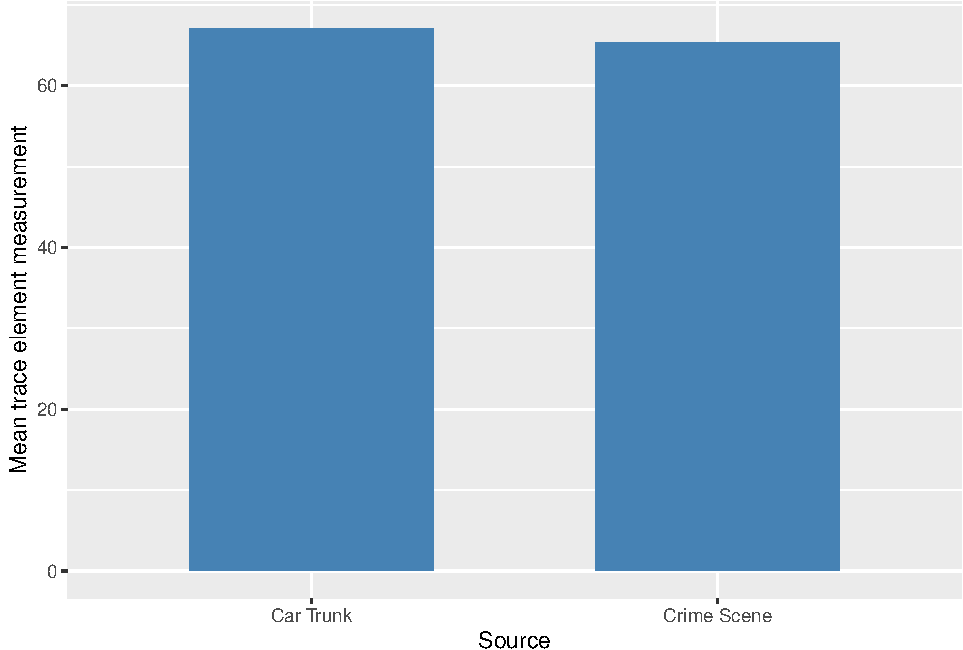
\includegraphics{forensic-statistics-book_files/figure-latex/bar-chart5-1.pdf}
\caption{\label{fig:bar-chart5}Comparison of mean trace element measurements}
\end{figure}

The heights of the bars are very similar, suggesting that there might be
a common source for the two sets of glass pieces. That might well be the
case but the means alone are not enough to provide a conclusion one way or
the other. In this case, box plots can be used instead since they provide
more information about the distribution. Figure \ref{fig:boxplot2a}
shows the box plots for this data again.

\begin{figure}
\centering
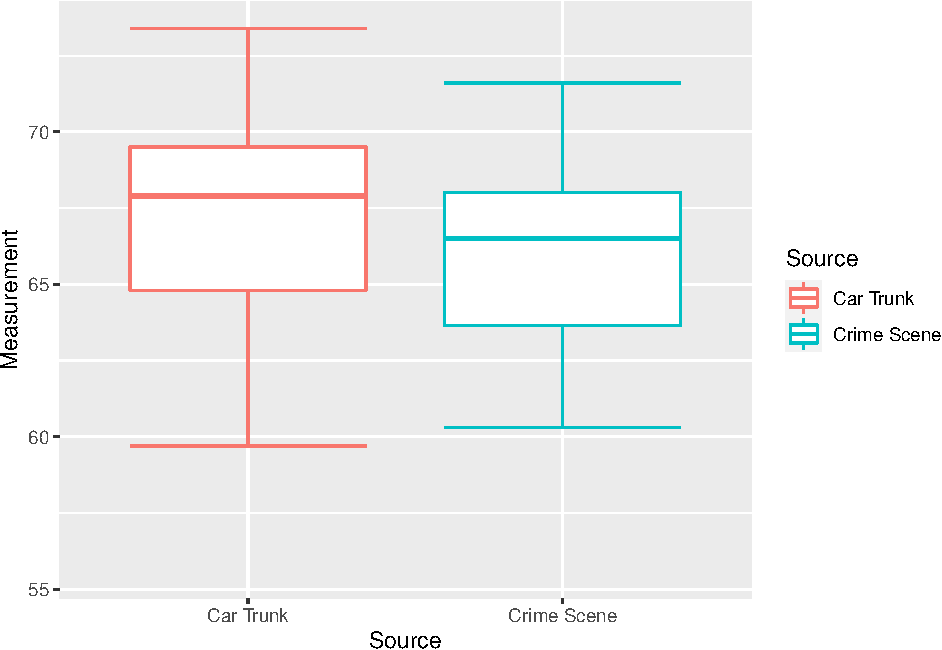
\includegraphics{forensic-statistics-book_files/figure-latex/boxplot2a-1.pdf}
\caption{\label{fig:boxplot2a}Box plots of glass measurements}
\end{figure}

The box plots have considerable overlap, but at the same time the middle 50\%
of values from the car trunk seem to trend higher than those from the crime
scene. This suggests the possibility of different sources for the two sets
of glass pieces while not ruling out the possibility of them coming from the
same source. We will consider this question more in later chapters.

\begin{center}\rule{0.5\linewidth}{0.5pt}\end{center}

\hypertarget{exercises-5}{%
\section{Exercises}\label{exercises-5}}

\begin{enumerate}
\def\labelenumi{\arabic{enumi}.}
\tightlist
\item
  \(\text{Put exercises here}\)
\end{enumerate}

\hypertarget{code-appendix-3}{%
\section{Code Appendix}\label{code-appendix-3}}

\begin{Shaded}
\begin{Highlighting}[]
\CommentTok{# Figure 10.1 -----}
\NormalTok{data <-}\StringTok{ }\KeywordTok{data.frame}\NormalTok{(}\DataTypeTok{ABO_Group =} \KeywordTok{c}\NormalTok{(}\StringTok{"A"}\NormalTok{, }\StringTok{"B"}\NormalTok{, }\StringTok{"AB"}\NormalTok{, }\StringTok{"O"}\NormalTok{), }\DataTypeTok{value =} \KeywordTok{c}\NormalTok{(}\DecValTok{210}\NormalTok{, }\DecValTok{45}\NormalTok{, }\DecValTok{15}\NormalTok{, }\DecValTok{230}\NormalTok{)) }\OperatorTok
\StringTok{  }\KeywordTok{mutate}\NormalTok{(}\DataTypeTok{prop =}\NormalTok{ value }\OperatorTok{/}\StringTok{ }\KeywordTok{sum}\NormalTok{(value) }\OperatorTok{*}\StringTok{ }\DecValTok{100}\NormalTok{)}

\KeywordTok{ggplot}\NormalTok{(data, }\KeywordTok{aes}\NormalTok{(ABO_Group, prop)) }\OperatorTok{+}\StringTok{ }
\StringTok{  }\KeywordTok{geom_bar}\NormalTok{(}\DataTypeTok{stat =} \StringTok{"identity"}\NormalTok{, }\DataTypeTok{fill =} \StringTok{"steelblue"}\NormalTok{, }\DataTypeTok{width =} \FloatTok{0.6}\NormalTok{) }\OperatorTok{+}\StringTok{ }
\StringTok{  }\KeywordTok{labs}\NormalTok{(}\DataTypeTok{x =} \StringTok{"ABO Group"}\NormalTok{, }\DataTypeTok{y =} \StringTok{"Percentage"}\NormalTok{)}

\CommentTok{# Figure 10.2 -----}
\NormalTok{data <-}\StringTok{ }\KeywordTok{data.frame}\NormalTok{(}\DataTypeTok{City =} \KeywordTok{c}\NormalTok{(}\StringTok{"Chicago"}\NormalTok{, }\StringTok{"Dallas"}\NormalTok{, }\StringTok{"Los Angeles"}\NormalTok{, }\StringTok{"New York"}\NormalTok{), }
                   \DataTypeTok{Murders =} \KeywordTok{c}\NormalTok{(}\DecValTok{774}\NormalTok{, }\DecValTok{251}\NormalTok{, }\DecValTok{349}\NormalTok{, }\DecValTok{468}\NormalTok{))}

\KeywordTok{ggplot}\NormalTok{(data, }\KeywordTok{aes}\NormalTok{(City, Murders)) }\OperatorTok{+}\StringTok{ }
\StringTok{  }\KeywordTok{geom_bar}\NormalTok{(}\DataTypeTok{stat =} \StringTok{"identity"}\NormalTok{, }\DataTypeTok{fill =} \StringTok{"steelblue"}\NormalTok{, }\DataTypeTok{width =} \FloatTok{0.6}\NormalTok{) }\OperatorTok{+}\StringTok{ }
\StringTok{  }\KeywordTok{labs}\NormalTok{(}\DataTypeTok{x =} \StringTok{"City"}\NormalTok{, }\DataTypeTok{y =} \StringTok{"Murders"}\NormalTok{)}

\CommentTok{# Figure 10.3 -----}
\NormalTok{data <-}\StringTok{ }\KeywordTok{data.frame}\NormalTok{(}\DataTypeTok{City =} \KeywordTok{c}\NormalTok{(}\StringTok{"Chicago"}\NormalTok{, }\StringTok{"Dallas"}\NormalTok{, }\StringTok{"Los Angeles"}\NormalTok{, }\StringTok{"New York"}\NormalTok{), }
                   \DataTypeTok{Murders =} \KeywordTok{c}\NormalTok{(}\FloatTok{281.8645}\NormalTok{, }\FloatTok{192.4847}\NormalTok{, }\FloatTok{89.51013}\NormalTok{, }\FloatTok{53.15766}\NormalTok{)) }

\KeywordTok{ggplot}\NormalTok{(data, }\KeywordTok{aes}\NormalTok{(City, Murders)) }\OperatorTok{+}\StringTok{ }
\StringTok{  }\KeywordTok{geom_bar}\NormalTok{(}\DataTypeTok{stat =} \StringTok{"identity"}\NormalTok{, }\DataTypeTok{fill =} \StringTok{"steelblue"}\NormalTok{, }\DataTypeTok{width =} \FloatTok{0.6}\NormalTok{) }\OperatorTok{+}\StringTok{ }
\StringTok{  }\KeywordTok{labs}\NormalTok{(}\DataTypeTok{x =} \StringTok{"City"}\NormalTok{, }\DataTypeTok{y =} \StringTok{"Murders per 1,000,000 residents"}\NormalTok{)}

\CommentTok{# Figure 10.4 -----}
\NormalTok{data <-}\StringTok{ }\KeywordTok{data.frame}\NormalTok{(}\DataTypeTok{City =} \KeywordTok{c}\NormalTok{(}\StringTok{"1995"}\NormalTok{, }\StringTok{"1996"}\NormalTok{, }\StringTok{"1997"}\NormalTok{, }\StringTok{"1998"}\NormalTok{, }\StringTok{"1999"}\NormalTok{, }\StringTok{"2000"}\NormalTok{), }
                   \DataTypeTok{RateChange =} \KeywordTok{c}\NormalTok{(}\FloatTok{62.7}\NormalTok{, }\FloatTok{41.3}\NormalTok{, }\FloatTok{-2.9}\NormalTok{, }\FloatTok{7.3}\NormalTok{, }\FloatTok{16.7}\NormalTok{, }\FloatTok{-6.7}\NormalTok{)) }

\CommentTok{# 2014-2020: 177, 288, 407, 395, 424, 495, 462 Shootings in Toronto (Wikipedia)}

\KeywordTok{ggplot}\NormalTok{(data, }\KeywordTok{aes}\NormalTok{(City, RateChange)) }\OperatorTok{+}\StringTok{ }
\StringTok{  }\KeywordTok{geom_bar}\NormalTok{(}\DataTypeTok{stat =} \StringTok{"identity"}\NormalTok{, }\DataTypeTok{fill =} \StringTok{"steelblue"}\NormalTok{, }\DataTypeTok{width =} \FloatTok{0.6}\NormalTok{) }\OperatorTok{+}\StringTok{ }
\StringTok{  }\KeywordTok{labs}\NormalTok{(}\DataTypeTok{x =} \StringTok{"Year"}\NormalTok{, }\DataTypeTok{y =} \StringTok{"Year-to-year Percent Change, Shootings"}\NormalTok{)}

\CommentTok{# Figure 10.5 -----}
\NormalTok{data01 =}\StringTok{ }\KeywordTok{c}\NormalTok{(}\FloatTok{55.6}\NormalTok{, }\FloatTok{65.6}\NormalTok{, }\FloatTok{68.0}\NormalTok{, }\FloatTok{68.9}\NormalTok{, }\FloatTok{67.7}\NormalTok{, }\FloatTok{66.5}\NormalTok{, }\FloatTok{66.8}\NormalTok{, }\FloatTok{60.3}\NormalTok{, }\FloatTok{68.0}\NormalTok{, }\FloatTok{71.6}\NormalTok{, }\FloatTok{61.4}\NormalTok{, }\FloatTok{63.2}\NormalTok{, }\FloatTok{68.2}\NormalTok{, }\FloatTok{64.1}\NormalTok{, }\FloatTok{64.8}\NormalTok{)}
\NormalTok{data02 =}\StringTok{ }\KeywordTok{c}\NormalTok{(}\FloatTok{67.9}\NormalTok{, }\FloatTok{68.9}\NormalTok{, }\FloatTok{69.5}\NormalTok{, }\FloatTok{67.6}\NormalTok{, }\FloatTok{73.4}\NormalTok{, }\FloatTok{64.5}\NormalTok{, }\FloatTok{73.0}\NormalTok{, }\FloatTok{59.7}\NormalTok{, }\FloatTok{66.9}\NormalTok{, }\FloatTok{68.2}\NormalTok{, }\FloatTok{71.8}\NormalTok{, }\FloatTok{64.8}\NormalTok{, }\FloatTok{56.3}\NormalTok{)}
\NormalTok{data <-}\StringTok{ }\KeywordTok{data.frame}\NormalTok{(}\DataTypeTok{Source =} \KeywordTok{c}\NormalTok{(}\StringTok{"Car Trunk"}\NormalTok{, }\StringTok{"Crime Scene"}\NormalTok{), }
                   \DataTypeTok{Mean =} \KeywordTok{c}\NormalTok{(}\KeywordTok{mean}\NormalTok{(data02), }\KeywordTok{mean}\NormalTok{(data01)))}

\KeywordTok{ggplot}\NormalTok{(data, }\KeywordTok{aes}\NormalTok{(Source, Mean)) }\OperatorTok{+}\StringTok{ }
\StringTok{  }\KeywordTok{geom_bar}\NormalTok{(}\DataTypeTok{stat =} \StringTok{"identity"}\NormalTok{, }\DataTypeTok{fill =} \StringTok{"steelblue"}\NormalTok{, }\DataTypeTok{width =} \FloatTok{0.6}\NormalTok{) }\OperatorTok{+}\StringTok{ }
\StringTok{  }\KeywordTok{labs}\NormalTok{(}\DataTypeTok{x =} \StringTok{"Source"}\NormalTok{, }\DataTypeTok{y =} \StringTok{"Mean trace element measurement"}\NormalTok{)}

\CommentTok{# Figure 10.6 -----}
\NormalTok{data01 <-}\StringTok{ }\KeywordTok{data.frame}\NormalTok{(}\DataTypeTok{Measurement =}\NormalTok{ data01, }\DataTypeTok{Source =} \StringTok{"Crime Scene"}\NormalTok{)}
\NormalTok{data02 <-}\StringTok{ }\KeywordTok{data.frame}\NormalTok{(}\DataTypeTok{Measurement =}\NormalTok{ data02, }\DataTypeTok{Source =} \StringTok{"Car Trunk"}\NormalTok{)}
\NormalTok{data03 =}\StringTok{ }\KeywordTok{rbind}\NormalTok{(data01, data02)}

\KeywordTok{ggplot}\NormalTok{(data03, }\KeywordTok{aes}\NormalTok{(}\DataTypeTok{x=}\NormalTok{Source, }\DataTypeTok{y=}\NormalTok{Measurement, }\DataTypeTok{color=}\NormalTok{Source)) }\OperatorTok{+}\StringTok{ }
\StringTok{  }\KeywordTok{stat_boxplot}\NormalTok{(}\DataTypeTok{geom =} \StringTok{"errorbar"}\NormalTok{) }\OperatorTok{+}\StringTok{ }\KeywordTok{geom_boxplot}\NormalTok{(}\DataTypeTok{outlier.shape =} \OtherTok{NA}\NormalTok{)}
\end{Highlighting}
\end{Shaded}

\hypertarget{sumarizing-distributions-central-tendency}{%
\chapter{Sumarizing Distributions: Central Tendency}\label{sumarizing-distributions-central-tendency}}

Note: Portions below modeled after content from
\emph{Online Statistics Education: A Multimedia Course of Study}
(\url{http://onlinestatbook.com/}) Project Leader: David M. Lane, Rice University

What is ``central tendency,'' and why do we want to know the central tendency of a group of scores? Let us first try to answer these questions intuitively. Then we will proceed to a more formal discussion.

\(\Sigma_{n=1}\)

Imagine this situation: You are in a class with just four other students, and the five of you took a 5-point pop quiz. Today your instructor is walking around the room, handing back the quizzes. She stops at your desk and hands you your paper. Written in bold black ink on the front is ``3/5.'' How do you react? Are you happy with your score of 3 or disappointed? How do you decide? You might calculate your percentage correct, realize it is 60\%, and be appalled. But it is more likely that when deciding how to react to your performance, you will want additional information. What additional information would you like?

If you are like most students, you will immediately ask your neighbors, ``Whad'ja get?'' and then ask the instructor, ``How did the class do?'' In other words, the additional information you want is how your quiz score compares to other students' scores. You therefore understand the importance of comparing your score to the class distribution of scores. Should your score of 3 turn out to be among the higher scores, then you'll be pleased after all. On the other hand, if 3 is among the lower scores in the class, you won't be quite so happy.

This idea of comparing individual scores to a distribution of scores is fundamental to statistics. So let's explore it further, using the same example (the pop quiz you took with your four classmates). Three possible outcomes are shown in Table 1. They are labeled ``Dataset A,'' ``Dataset B,'' and ``Dataset C.'' Which of the three datasets would make you happiest? In other words, in comparing your score with your fellow students' scores, in which dataset would your score of 3 be the most impressive?

In Dataset A, everyone's score is 3. This puts your score at the exact center of the distribution. You can draw satisfaction from the fact that you did as well as everyone else. But of course it cuts both ways: everyone else did just as well as you.

Table 1. Three possible datasets for the 5-point make-up quiz.

Student Dataset A Dataset B Dataset C
You 3 3 3
John's 3 4 2
Maria's 3 4 2
Shareecia's 3 4 2
Luther's 3 5 1
Now consider the possibility that the scores are described as in Dataset B. This is a depressing outcome even though your score is no different than the one in Dataset A. The problem is that the other four students had higher grades, putting yours below the center of the distribution.

Finally, let's look at Dataset C. This is more like it! All of your classmates score lower than you so your score is above the center of the distribution.

Now let's change the example in order to develop more insight into the center of a distribution. Figure 1 shows the results of an experiment on memory for chess positions. Subjects were shown a chess position and then asked to reconstruct it on an empty chess board. The number of pieces correctly placed was recorded. This was repeated for two more chess positions. The scores represent the total number of chess pieces correctly placed for the three chess positions. The maximum possible score was 89.

Two groups are compared. On the left are people who don't play chess. On the right are people who play a great deal (tournament players). It is clear that the location of the center of the distribution for the non-players is much lower than the center of the distribution for the tournament players.

Figure 1. Back-to-back stem and leaf display. The left side shows the memory scores of the non-players. The right side shows the scores of the tournament players.

We're sure you get the idea now about the center of a distribution. It is time to move beyond intuition. We need a formal definition of the center of a distribution. In fact, we'll offer you three definitions! This is not just generosity on our part. There turn out to be (at least) three different ways of thinking about the center of a distribution, all of them useful in various contexts. In the remainder of this section we attempt to communicate the idea behind each concept. In the succeeding sections we will give statistical measures for these concepts of central tendency.

Definitions of Center

Now we explain the three different ways of defining the center of a distribution. All three are called measures of central tendency.

Balance Scale

One definition of central tendency is the point at which the distribution is in balance. Figure 2 shows the distribution of the five numbers 2, 3, 4, 9, 16 placed upon a balance scale. If each number weighs one pound, and is placed at its position along the number line, then it would be possible to balance them by placing a fulcrum at 6.8.

Figure 2. A balance scale.

For another example, consider the distribution shown in Figure 3. It is balanced by placing the fulcrum in the geometric middle.

Figure 3. A distribution balanced on the tip of a triangle.

Figure 4 illustrates that the same distribution can't be balanced by placing the fulcrum to the left of center.

Figure 4. The distribution is not balanced.

Figure 5 shows an asymmetric distribution. To balance it, we cannot put the fulcrum halfway between the lowest and highest values (as we did in Figure 3). Placing the fulcrum at the ``half way'' point would cause it to tip towards the left.

Figure 5. An asymmetric distribution balanced on the tip of a triangle.

The balance point defines one sense of a distribution's center. The simulation in the next section ``Balance Scale Simulation'' shows how to find the point at which the distribution balances.

Smallest Absolute Deviation

Another way to define the center of a distribution is based on the concept of the sum of the absolute deviations (differences). Consider the distribution made up of the five numbers 2, 3, 4, 9, 16. Let's see how far the distribution is from 10 (picking a number arbitrarily). Table 2 shows the sum of the absolute deviations of these numbers from the number 10.

Table 2. An example of the sum of absolute deviations

Values Absolute Deviations from 10
2
3
4
9
16 8
7
6
1
6
Sum 28
The first row of the table shows that the absolute value of the difference between 2 and 10 is 8; the second row shows that the absolute difference between 3 and 10 is 7, and similarly for the other rows. When we add up the five absolute deviations, we get 28. So, the sum of the absolute deviations from 10 is 28. Likewise, the sum of the absolute deviations from 5 equals 3 + 2 + 1 + 4 + 11 = 21. So, the sum of the absolute deviations from 5 is smaller than the sum of the absolute deviations from 10. In this sense, 5 is closer, overall, to the other numbers than is 10.

We are now in a position to define a second measure of central tendency, this time in terms of absolute deviations. Specifically, according to our second definition, the center of a distribution is the number for which the sum of the absolute deviations is smallest. As we just saw, the sum of the absolute deviations from 10 is 28 and the sum of the absolute deviations from 5 is 21. Is there a value for which the sum of the absolute deviations is even smaller than 21? Yes. For these data, there is a value for which the sum of absolute deviations is only 20. See if you can find it. A general method for finding the center of a distribution in the sense of absolute deviations is provided in the simulation ``Absolute Differences Simulation.''

Smallest Squared Deviation

We shall discuss one more way to define the center of a distribution. It is based on the concept of the sum of squared deviations (differences). Again, consider the distribution of the five numbers 2, 3, 4, 9, 16. Table 3 shows the sum of the squared deviations of these numbers from the number 10.

Table 3. An example of the sum of squared deviations.

Values Squared Deviations
from 10
2
3
4
9
16 64
49
36
1
36
Sum 186
The first row in the table shows that the squared value of the difference between 2 and 10 is 64; the second row shows that the squared difference between 3 and 10 is 49, and so forth. When we add up all these squared deviations, we get 186. Changing the target from 10 to 5, we calculate the sum of the squared deviations from 5 as 9 + 4 + 1 + 16 + 121 = 151. So, the sum of the squared deviations from 5 is smaller than the sum of the squared deviations from 10. Is there a value for which the sum of the squared deviations is even smaller than 151? Yes, it is possible to reach 134.8. Can you find the target number for which the sum of squared deviations is 134.8?

The target that minimizes the sum of squared deviations provides another useful definition of central tendency (the last one to be discussed in this section). It can be challenging to find the value that minimizes this sum. You will see how you do it in the upcoming section ``Squared Differences Simulation.''

\begin{center}\rule{0.5\linewidth}{0.5pt}\end{center}

\hypertarget{exercises-6}{%
\section{Exercises}\label{exercises-6}}

\begin{enumerate}
\def\labelenumi{\arabic{enumi}.}
\tightlist
\item
  \(\text{Put exercises here}\)
\end{enumerate}

\hypertarget{sumarizing-distributions-measures-of-central-tendency}{%
\chapter{Sumarizing Distributions: Measures of Central Tendency}\label{sumarizing-distributions-measures-of-central-tendency}}

Note: Portions below modeled after content from
\emph{Online Statistics Education: A Multimedia Course of Study}
(\url{http://onlinestatbook.com/}) Project Leader: David M. Lane, Rice University

In the previous section we saw that there are several ways to define central tendency. This section defines the three most common measures of central tendency: the mean, the median, and the mode. The relationships among these measures of central tendency and the definitions given in the previous section will probably not be obvious to you. Rather than just tell you these relationships, we will allow you to discover them in the simulations in the sections that follow.

This section gives only the basic definitions of the mean, median and mode. A further discussion of the relative merits and proper applications of these statistics is presented in a later section.

Arithmetic Mean

The arithmetic mean is the most common measure of central tendency. It is simply the sum of the numbers divided by the number of numbers. The symbol ``μ'' is used for the mean of a population. The symbol ``M'' is used for the mean of a sample. The formula for μ is shown below:

μ = ΣX/N
where ΣX is the sum of all the numbers in the population and
N is the number of numbers in the population.

The formula for M is essentially identical:

M = ΣX/N
where ΣX is the sum of all the numbers in the sample and
N is the number of numbers in the sample.

As an example, the mean of the numbers 1, 2, 3, 6, 8 is 20/5 = 4 regardless of whether the numbers constitute the entire population or just a sample from the population.

Table 1 shows the number of touchdown (TD) passes thrown by each of the 31 teams in the National Football League in the 2000 season. The mean number of touchdown passes thrown is 20.4516 as shown below.

μ = ΣX/N
= 634/31
= 20.4516
Table 1. Number of touchdown passes.

37 33 33 32 29 28 28 23 22 22 22 21 21 21 20 20 19 19 18 18 18 18 16 15 14 14 14 12 12 9 6
Although the arithmetic mean is not the only ``mean'' (there is also a geometric mean), it is by far the most commonly used. Therefore, if the term ``mean'' is used without specifying whether it is the arithmetic mean, the geometric mean, or some other mean, it is assumed to refer to the arithmetic mean.

Median

The median is also a frequently used measure of central tendency. The median is the midpoint of a distribution: the same number of scores is above the median as below it. For the data in Table 1, there are 31 scores. The 16th highest score (which equals 20) is the median because there are 15 scores below the 16th score and 15 scores above the 16th score. The median can also be thought of as the 50th percentile.

Computation of the Median

When there is an odd number of numbers, the median is simply the middle number. For example, the median of 2, 4, and 7 is 4. When there is an even number of numbers, the median is the mean of the two middle numbers. Thus, the median of the numbers 2, 4, 7, 12 is (4+7)/2 = 5.5. When there are numbers with the same values, then the formula for the third definition of the 50th percentile should be used.

Mode

The mode is the most frequently occurring value. For the data in Table 1, the mode is 18 since more teams (4) had 18 touchdown passes than any other number of touchdown passes. With continuous data such as response time measured to many decimals, the frequency of each value is one since no two scores will be exactly the same (see discussion of continuous variables). Therefore the mode of continuous data is normally computed from a grouped frequency distribution. Table 2 shows a grouped frequency distribution for the target response time data. Since the interval with the highest frequency is 600-700, the mode is the middle of that interval (650).

Table 2. Grouped frequency distribution.

Range Frequency
500-600
600-700
700-800
800-900
900-1000
1000-1100 3
6
5
5
0
1

\begin{center}\rule{0.5\linewidth}{0.5pt}\end{center}

\hypertarget{exercises-7}{%
\section{Exercises}\label{exercises-7}}

\begin{enumerate}
\def\labelenumi{\arabic{enumi}.}
\tightlist
\item
  \(\text{Put exercises here}\)
\end{enumerate}

  \bibliography{book.bib,packages.bib}

\end{document}
